\documentclass[a4paper]{book}
\usepackage{makeidx}
\usepackage{graphicx}
\usepackage{multicol}
\usepackage{float}
\usepackage{listings}
\usepackage{color}
\usepackage{ifthen}
\usepackage[table]{xcolor}
\usepackage{textcomp}
\usepackage{alltt}
\usepackage{ifpdf}
\ifpdf
\usepackage[pdftex,
            pagebackref=true,
            colorlinks=true,
            linkcolor=blue,
            unicode
           ]{hyperref}
\else
\usepackage[ps2pdf,
            pagebackref=true,
            colorlinks=true,
            linkcolor=blue,
            unicode
           ]{hyperref}
\usepackage{pspicture}
\fi
\usepackage[utf8]{inputenc}
\usepackage[french]{babel}

\usepackage{mathptmx}
\usepackage[scaled=.90]{helvet}
\usepackage{courier}
\usepackage{doxygen}
\lstset{language=C++,inputencoding=utf8,basicstyle=\footnotesize,breaklines=true,breakatwhitespace=true,tabsize=8,numbers=left }
\makeindex
\setcounter{tocdepth}{3}
\renewcommand{\footrulewidth}{0.4pt}
\begin{document}
\hypersetup{pageanchor=false}
\begin{titlepage}
\vspace*{7cm}
\begin{center}
{\Large Jeu de dames \\[1ex]\large Version Finale }\\
\vspace*{1cm}
{\large Généré par Doxygen 1.7.3}\\
\vspace*{0.5cm}
{\small Mon May 9 2011 00:36:50}\\
\end{center}
\end{titlepage}
\clearemptydoublepage
\pagenumbering{roman}
\tableofcontents
\clearemptydoublepage
\pagenumbering{arabic}
\hypersetup{pageanchor=true}
\chapter{Index des structures de données}
\section{Structures de données}
Liste des structures de données avec une brève description :\begin{DoxyCompactList}
\item\contentsline{section}{\hyperlink{structarbre}{arbre} (Un arbre à une valeur (la racine) et un certain nombre de fils )}{\pageref{structarbre}}{}
\item\contentsline{section}{\hyperlink{struct_carre__clair}{Carre\_\-clair} }{\pageref{struct_carre__clair}}{}
\item\contentsline{section}{\hyperlink{struct_carre__fonce}{Carre\_\-fonce} }{\pageref{struct_carre__fonce}}{}
\item\contentsline{section}{\hyperlink{structcase__plateau}{case\_\-plateau} (Objet case du plateau de jeu. Une case est définie par une couleur et, si elle est noire,elle dispose d'une abscisse (x) et une ordonnée (y) sur le plateau. Une case peut être libre ou non, si elle n'est pas libre elle contient un pion )}{\pageref{structcase__plateau}}{}
\item\contentsline{section}{\hyperlink{structcoup}{coup} (Objet coup. Un coup est défini par un numéro de case de départ, un numéro de case d'arrivée, un type (déplacement ou prise) et optinellement un commentaire )}{\pageref{structcoup}}{}
\item\contentsline{section}{\hyperlink{structjoueur}{joueur} (Objet joueur. Un joueur est caractérisé par la couleur qu'il joue et sa nature (humain ou intelligence artificielle) )}{\pageref{structjoueur}}{}
\item\contentsline{section}{\hyperlink{structpion}{pion} (Objet pion. Un pion est déterminé par une couleur et si il est une dame ou non )}{\pageref{structpion}}{}
\item\contentsline{section}{\hyperlink{struct_pion__clair}{Pion\_\-clair} }{\pageref{struct_pion__clair}}{}
\item\contentsline{section}{\hyperlink{struct_pion__fonce}{Pion\_\-fonce} }{\pageref{struct_pion__fonce}}{}
\item\contentsline{section}{\hyperlink{structplateau}{plateau} (Objet plateau. Le plateau est composé de 50 cases, numérotées de 1 à 50. Il comporte un historique des coups. Il sait quel joueur doit jouer le prochain coup )}{\pageref{structplateau}}{}
\end{DoxyCompactList}

\chapter{Index des fichiers}
\section{Liste des fichiers}
Liste de tous les fichiers documentés avec une brève description :\begin{DoxyCompactList}
\item\contentsline{section}{{\bfseries arbre.c} }{\pageref{arbre_8c}}{}
\item\contentsline{section}{\hyperlink{arbre_8h}{arbre.h} (Implémantation des arbres )}{\pageref{arbre_8h}}{}
\item\contentsline{section}{\hyperlink{constantes_8h}{constantes.h} (Constantes utiles pour l'interface )}{\pageref{constantes_8h}}{}
\item\contentsline{section}{{\bfseries fonction\_\-evaluation.c} }{\pageref{fonction__evaluation_8c}}{}
\item\contentsline{section}{\hyperlink{fonction__evaluation_8h}{fonction\_\-evaluation.h} (La fonction d'evaluation de l'algorithme MinMax. Renvoie un double compris entre -\/1 et 1 caracterisant un etat du plateau plus ou moins favorable au joueur courant )}{\pageref{fonction__evaluation_8h}}{}
\item\contentsline{section}{{\bfseries fonctionInterface.c} }{\pageref{fonction_interface_8c}}{}
\item\contentsline{section}{\hyperlink{fonction_interface_8h}{fonctionInterface.h} (Implémentation de fonctionnalités pour l'interface )}{\pageref{fonction_interface_8h}}{}
\item\contentsline{section}{{\bfseries main.c} }{\pageref{main_8c}}{}
\item\contentsline{section}{{\bfseries min-\/max.c} }{\pageref{min-max_8c}}{}
\item\contentsline{section}{\hyperlink{min-max_8h}{min-\/max.h} (Implémentation du min-\/max )}{\pageref{min-max_8h}}{}
\item\contentsline{section}{{\bfseries moteur.c} }{\pageref{moteur_8c}}{}
\item\contentsline{section}{\hyperlink{moteur_8h}{moteur.h} (Le moteur de jeu. Il permet de gérer une partie, 1 ou 2 joueurs, fait jouer l'IA, fournit une aide au joueur )}{\pageref{moteur_8h}}{}
\item\contentsline{section}{{\bfseries plateau.c} }{\pageref{plateau_8c}}{}
\item\contentsline{section}{\hyperlink{plateau_8h}{plateau.h} (Tout ce qui concerne le plateau de jeu (damier, pions et joueurs) )}{\pageref{plateau_8h}}{}
\item\contentsline{section}{{\bfseries regles.c} }{\pageref{regles_8c}}{}
\item\contentsline{section}{\hyperlink{regles_8h}{regles.h} (Module des regles et d'enumeration des coups )}{\pageref{regles_8h}}{}
\end{DoxyCompactList}

\chapter{Documentation des structures de données}
\hypertarget{structarbre}{
\section{Référence de la structure arbre}
\label{structarbre}\index{arbre@{arbre}}
}


Un arbre à une valeur (la racine) et un certain nombre de fils.  




{\ttfamily \#include $<$arbre.h$>$}



Graphe de collaboration de arbre:\nopagebreak
\begin{figure}[H]
\begin{center}
\leavevmode
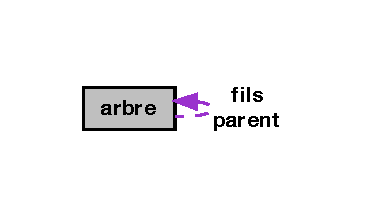
\includegraphics[width=176pt]{structarbre__coll__graph}
\end{center}
\end{figure}
\subsection*{Champs de données}
\begin{DoxyCompactItemize}
\item 
\hypertarget{structarbre_a4a8f7bc357d6e8bff6aa5eee7a166f81}{
struct \hyperlink{structarbre}{arbre} $\ast$ {\bfseries parent}}
\label{structarbre_a4a8f7bc357d6e8bff6aa5eee7a166f81}

\item 
\hypertarget{structarbre_a8e030c012e3b74a6d076739c4c7ecb69}{
int {\bfseries valeur}}
\label{structarbre_a8e030c012e3b74a6d076739c4c7ecb69}

\item 
\hypertarget{structarbre_aa9b3fa948258da2518cebbe8cb191431}{
int {\bfseries profondeur}}
\label{structarbre_aa9b3fa948258da2518cebbe8cb191431}

\item 
int \hyperlink{structarbre_a67c44f020d501282adc38e3301a5f245}{nb\_\-fils}
\item 
struct \hyperlink{structarbre}{arbre} $\ast$ \hyperlink{structarbre_a7bac08e3c2aedbde0dddf80b94eadf76}{fils} \mbox{[}80\mbox{]}
\end{DoxyCompactItemize}


\subsection{Description détaillée}
Un arbre à une valeur (la racine) et un certain nombre de fils. 

Définition à la ligne \hyperlink{arbre_8h_source_l00013}{13} du fichier \hyperlink{arbre_8h_source}{arbre.h}.



\subsection{Documentation des champs}
\hypertarget{structarbre_a7bac08e3c2aedbde0dddf80b94eadf76}{
\index{arbre@{arbre}!fils@{fils}}
\index{fils@{fils}!arbre@{arbre}}
\subsubsection[{fils}]{\setlength{\rightskip}{0pt plus 5cm}struct {\bf arbre}$\ast$ {\bf fils}\mbox{[}80\mbox{]}}}
\label{structarbre_a7bac08e3c2aedbde0dddf80b94eadf76}
Un noeud n'aura jamais plus de 80 fils car on a, pour un demi-\/coup, 20 pions $\ast$ 4 déplacements possibles = 80 coups différents. 

Définition à la ligne \hyperlink{arbre_8h_source_l00018}{18} du fichier \hyperlink{arbre_8h_source}{arbre.h}.

\hypertarget{structarbre_a67c44f020d501282adc38e3301a5f245}{
\index{arbre@{arbre}!nb\_\-fils@{nb\_\-fils}}
\index{nb\_\-fils@{nb\_\-fils}!arbre@{arbre}}
\subsubsection[{nb\_\-fils}]{\setlength{\rightskip}{0pt plus 5cm}int {\bf nb\_\-fils}}}
\label{structarbre_a67c44f020d501282adc38e3301a5f245}
Le nombre de fils de ce noeud 

Définition à la ligne \hyperlink{arbre_8h_source_l00017}{17} du fichier \hyperlink{arbre_8h_source}{arbre.h}.



La documentation de cette structure a été générée à partir du fichier suivant :\begin{DoxyCompactItemize}
\item 
\hyperlink{arbre_8h}{arbre.h}\end{DoxyCompactItemize}

\hypertarget{struct_carre__clair}{
\section{Référence de la structure Carre\_\-clair}
\label{struct_carre__clair}\index{Carre\_\-clair@{Carre\_\-clair}}
}


{\ttfamily \#include $<$constantes.h$>$}

\subsection*{Champs de données}
\begin{DoxyCompactItemize}
\item 
\hypertarget{struct_carre__clair_a173f25d2fd7c653d77ca8174ba4f636d}{
int {\bfseries est\_\-libre}}
\label{struct_carre__clair_a173f25d2fd7c653d77ca8174ba4f636d}

\item 
\hypertarget{struct_carre__clair_ae7469189d260b9609e5e1c4d1b0b7ed4}{
int {\bfseries numero\_\-case}}
\label{struct_carre__clair_ae7469189d260b9609e5e1c4d1b0b7ed4}

\item 
\hypertarget{struct_carre__clair_ac06cf6a292dc0e70e28b394fa481aef2}{
SDL\_\-Rect {\bfseries position}}
\label{struct_carre__clair_ac06cf6a292dc0e70e28b394fa481aef2}

\item 
\hypertarget{struct_carre__clair_a2f5cac12e913bcfcff660305bf88dd3b}{
SDL\_\-Surface $\ast$ {\bfseries surface}}
\label{struct_carre__clair_a2f5cac12e913bcfcff660305bf88dd3b}

\end{DoxyCompactItemize}


\subsection{Description détaillée}
Structure definissant un carre clair 

Définition à la ligne \hyperlink{constantes_8h_source_l00037}{37} du fichier \hyperlink{constantes_8h_source}{constantes.h}.



La documentation de cette structure a été générée à partir du fichier suivant :\begin{DoxyCompactItemize}
\item 
\hyperlink{constantes_8h}{constantes.h}\end{DoxyCompactItemize}

\hypertarget{struct_carre__fonce}{
\section{Référence de la structure Carre\_\-fonce}
\label{struct_carre__fonce}\index{Carre\_\-fonce@{Carre\_\-fonce}}
}


{\ttfamily \#include $<$constantes.h$>$}

\subsection*{Champs de données}
\begin{DoxyCompactItemize}
\item 
\hypertarget{struct_carre__fonce_a173f25d2fd7c653d77ca8174ba4f636d}{
int {\bfseries est\_\-libre}}
\label{struct_carre__fonce_a173f25d2fd7c653d77ca8174ba4f636d}

\item 
\hypertarget{struct_carre__fonce_ae7469189d260b9609e5e1c4d1b0b7ed4}{
int {\bfseries numero\_\-case}}
\label{struct_carre__fonce_ae7469189d260b9609e5e1c4d1b0b7ed4}

\item 
\hypertarget{struct_carre__fonce_ac06cf6a292dc0e70e28b394fa481aef2}{
SDL\_\-Rect {\bfseries position}}
\label{struct_carre__fonce_ac06cf6a292dc0e70e28b394fa481aef2}

\item 
\hypertarget{struct_carre__fonce_a2f5cac12e913bcfcff660305bf88dd3b}{
SDL\_\-Surface $\ast$ {\bfseries surface}}
\label{struct_carre__fonce_a2f5cac12e913bcfcff660305bf88dd3b}

\end{DoxyCompactItemize}


\subsection{Description détaillée}
Structure definissant un carre fonce 

Définition à la ligne \hyperlink{constantes_8h_source_l00029}{29} du fichier \hyperlink{constantes_8h_source}{constantes.h}.



La documentation de cette structure a été générée à partir du fichier suivant :\begin{DoxyCompactItemize}
\item 
\hyperlink{constantes_8h}{constantes.h}\end{DoxyCompactItemize}

\hypertarget{structcase__plateau}{
\section{Référence de la structure case\_\-plateau}
\label{structcase__plateau}\index{case\_\-plateau@{case\_\-plateau}}
}


Objet case du plateau de jeu. Une case est définie par une couleur et, si elle est noire,elle dispose d'une abscisse (x) et une ordonnée (y) sur le plateau. Une case peut être libre ou non, si elle n'est pas libre elle contient un pion.  




{\ttfamily \#include $<$plateau.h$>$}



Graphe de collaboration de case\_\-plateau:\nopagebreak
\begin{figure}[H]
\begin{center}
\leavevmode
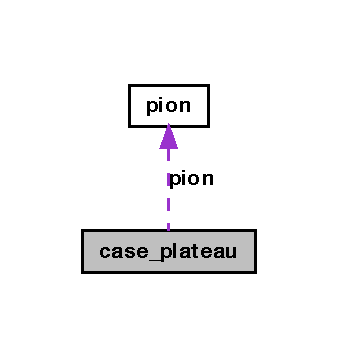
\includegraphics[width=162pt]{structcase__plateau__coll__graph}
\end{center}
\end{figure}
\subsection*{Champs de données}
\begin{DoxyCompactItemize}
\item 
\hyperlink{plateau_8h_a8282be6127518547fa916dd6cfef17cb}{couleur\_\-pion} \hyperlink{structcase__plateau_a057f95a41503a890f27c651969ffac8d}{couleur}
\item 
int \hyperlink{structcase__plateau_a173f25d2fd7c653d77ca8174ba4f636d}{est\_\-libre}
\item 
\hypertarget{structcase__plateau_a8bae207c875a01f3370c58bd07b8fa82}{
\hyperlink{structpion}{pion} {\bfseries pion}}
\label{structcase__plateau_a8bae207c875a01f3370c58bd07b8fa82}

\item 
\hypertarget{structcase__plateau_a6150e0515f7202e2fb518f7206ed97dc}{
int {\bfseries x}}
\label{structcase__plateau_a6150e0515f7202e2fb518f7206ed97dc}

\item 
\hypertarget{structcase__plateau_a0a2f84ed7838f07779ae24c5a9086d33}{
int {\bfseries y}}
\label{structcase__plateau_a0a2f84ed7838f07779ae24c5a9086d33}

\item 
int \hyperlink{structcase__plateau_ad510581b324604a9cf685cbb769a421a}{notation\_\-officielle}
\item 
int \hyperlink{structcase__plateau_ae49bb71ca6836b02fd9efa3c1fa64405}{en\_\-surbrillance}
\end{DoxyCompactItemize}


\subsection{Description détaillée}
Objet case du plateau de jeu. Une case est définie par une couleur et, si elle est noire,elle dispose d'une abscisse (x) et une ordonnée (y) sur le plateau. Une case peut être libre ou non, si elle n'est pas libre elle contient un pion. 

Définition à la ligne \hyperlink{plateau_8h_source_l00045}{45} du fichier \hyperlink{plateau_8h_source}{plateau.h}.



\subsection{Documentation des champs}
\hypertarget{structcase__plateau_a057f95a41503a890f27c651969ffac8d}{
\index{case\_\-plateau@{case\_\-plateau}!couleur@{couleur}}
\index{couleur@{couleur}!case_plateau@{case\_\-plateau}}
\subsubsection[{couleur}]{\setlength{\rightskip}{0pt plus 5cm}{\bf couleur\_\-pion} {\bf couleur}}}
\label{structcase__plateau_a057f95a41503a890f27c651969ffac8d}
La couleur de la case. 

Définition à la ligne \hyperlink{plateau_8h_source_l00046}{46} du fichier \hyperlink{plateau_8h_source}{plateau.h}.

\hypertarget{structcase__plateau_ae49bb71ca6836b02fd9efa3c1fa64405}{
\index{case\_\-plateau@{case\_\-plateau}!en\_\-surbrillance@{en\_\-surbrillance}}
\index{en\_\-surbrillance@{en\_\-surbrillance}!case_plateau@{case\_\-plateau}}
\subsubsection[{en\_\-surbrillance}]{\setlength{\rightskip}{0pt plus 5cm}int {\bf en\_\-surbrillance}}}
\label{structcase__plateau_ae49bb71ca6836b02fd9efa3c1fa64405}
Si la case doit être affichée en surbrillance. 

Définition à la ligne \hyperlink{plateau_8h_source_l00052}{52} du fichier \hyperlink{plateau_8h_source}{plateau.h}.

\hypertarget{structcase__plateau_a173f25d2fd7c653d77ca8174ba4f636d}{
\index{case\_\-plateau@{case\_\-plateau}!est\_\-libre@{est\_\-libre}}
\index{est\_\-libre@{est\_\-libre}!case_plateau@{case\_\-plateau}}
\subsubsection[{est\_\-libre}]{\setlength{\rightskip}{0pt plus 5cm}int {\bf est\_\-libre}}}
\label{structcase__plateau_a173f25d2fd7c653d77ca8174ba4f636d}
Vrai si la case est vide 

Définition à la ligne \hyperlink{plateau_8h_source_l00047}{47} du fichier \hyperlink{plateau_8h_source}{plateau.h}.

\hypertarget{structcase__plateau_ad510581b324604a9cf685cbb769a421a}{
\index{case\_\-plateau@{case\_\-plateau}!notation\_\-officielle@{notation\_\-officielle}}
\index{notation\_\-officielle@{notation\_\-officielle}!case_plateau@{case\_\-plateau}}
\subsubsection[{notation\_\-officielle}]{\setlength{\rightskip}{0pt plus 5cm}int {\bf notation\_\-officielle}}}
\label{structcase__plateau_ad510581b324604a9cf685cbb769a421a}
Le numéro de la case selon la notation officielle. 

Définition à la ligne \hyperlink{plateau_8h_source_l00051}{51} du fichier \hyperlink{plateau_8h_source}{plateau.h}.



La documentation de cette structure a été générée à partir du fichier suivant :\begin{DoxyCompactItemize}
\item 
\hyperlink{plateau_8h}{plateau.h}\end{DoxyCompactItemize}

\hypertarget{structcoup}{
\section{Référence de la structure coup}
\label{structcoup}\index{coup@{coup}}
}


Objet coup. Un coup est défini par un numéro de case de départ, un numéro de case d'arrivée, un type (déplacement ou prise) et optinellement un commentaire.  




{\ttfamily \#include $<$plateau.h$>$}



Graphe de collaboration de coup:\nopagebreak
\begin{figure}[H]
\begin{center}
\leavevmode
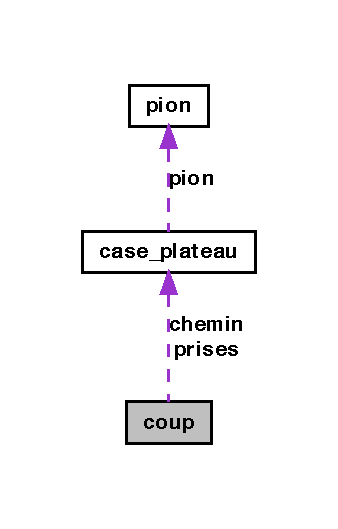
\includegraphics[width=162pt]{structcoup__coll__graph}
\end{center}
\end{figure}
\subsection*{Champs de données}
\begin{DoxyCompactItemize}
\item 
\hypertarget{structcoup_a7d3cdc0f60034d9940699758db062357}{
int {\bfseries old\_\-case}}
\label{structcoup_a7d3cdc0f60034d9940699758db062357}

\item 
\hypertarget{structcoup_a59e06844f696ebfa6d06977d60276514}{
int {\bfseries new\_\-case}}
\label{structcoup_a59e06844f696ebfa6d06977d60276514}

\item 
\hyperlink{plateau_8h_a9e00f85b4b6ec2d8bdfbe94ff40f0eee}{type\_\-coup} \hyperlink{structcoup_aa33da004dccb192cb33bc00c26c6e859}{tc}
\item 
\hypertarget{structcoup_a8c9c2c766a89b66caa7117708f247b2d}{
int {\bfseries nombre\_\-prises}}
\label{structcoup_a8c9c2c766a89b66caa7117708f247b2d}

\item 
\hyperlink{structcase__plateau}{case\_\-plateau} \hyperlink{structcoup_ae19b3a66d3f4e66b8f69a38e4005f44a}{prises} \mbox{[}20\mbox{]}
\item 
\hyperlink{structcase__plateau}{case\_\-plateau} \hyperlink{structcoup_aa66b88eb8140c2f459ac92fad0796510}{chemin} \mbox{[}20\mbox{]}
\item 
char $\ast$ \hyperlink{structcoup_a8978a8d22b339f32c70e5cb900d4c961}{commentaire}
\end{DoxyCompactItemize}


\subsection{Description détaillée}
Objet coup. Un coup est défini par un numéro de case de départ, un numéro de case d'arrivée, un type (déplacement ou prise) et optinellement un commentaire. 

Définition à la ligne \hyperlink{plateau_8h_source_l00074}{74} du fichier \hyperlink{plateau_8h_source}{plateau.h}.



\subsection{Documentation des champs}
\hypertarget{structcoup_aa66b88eb8140c2f459ac92fad0796510}{
\index{coup@{coup}!chemin@{chemin}}
\index{chemin@{chemin}!coup@{coup}}
\subsubsection[{chemin}]{\setlength{\rightskip}{0pt plus 5cm}{\bf case\_\-plateau} {\bf chemin}\mbox{[}20\mbox{]}}}
\label{structcoup_aa66b88eb8140c2f459ac92fad0796510}
Liste de cases sur lesquelles le pion s'arrête lors d'une rafle (pour repérer la fin de liste, la dernière case sera une case blanche). 

Définition à la ligne \hyperlink{plateau_8h_source_l00080}{80} du fichier \hyperlink{plateau_8h_source}{plateau.h}.

\hypertarget{structcoup_a8978a8d22b339f32c70e5cb900d4c961}{
\index{coup@{coup}!commentaire@{commentaire}}
\index{commentaire@{commentaire}!coup@{coup}}
\subsubsection[{commentaire}]{\setlength{\rightskip}{0pt plus 5cm}char$\ast$ {\bf commentaire}}}
\label{structcoup_a8978a8d22b339f32c70e5cb900d4c961}
Les commentaires sont :\par
 \begin{DoxyItemize}
\item ! pour indiquer un coup fort ou bien joué\par
 \item !! pour indiquer un coup très fort\par
 \item ? pour indiquer un coup faible ou mal joué\par
 \item ?? pour indiquer un coup très faible ou une gaffe\par
 \item !? pour indiquer un coup paraissant fort, mais qui en réalité se révèle faible\par
 \item ?! pour indiquer un coup paraissant faible, mais qui en réalité se révèle fort\par
 \item $\ast$ pour indiquer un coup forcé, tout autre mouvement entraînant une perte immédiate\par
 \item + pour indiquer le gain de la partie\par
 \item = pour indiquer un jeu égal\par
 \item +1 pour indiquer le gain d’un pion\par
 \item +n pour indiquer le gain de n pion\par
 \item +-\/ pour indiquer un avantage aux blancs\par
 \item -\/+ pour indiquer un avantage aux noirs \end{DoxyItemize}


Définition à la ligne \hyperlink{plateau_8h_source_l00082}{82} du fichier \hyperlink{plateau_8h_source}{plateau.h}.

\hypertarget{structcoup_ae19b3a66d3f4e66b8f69a38e4005f44a}{
\index{coup@{coup}!prises@{prises}}
\index{prises@{prises}!coup@{coup}}
\subsubsection[{prises}]{\setlength{\rightskip}{0pt plus 5cm}{\bf case\_\-plateau} {\bf prises}\mbox{[}20\mbox{]}}}
\label{structcoup_ae19b3a66d3f4e66b8f69a38e4005f44a}
Les cases sur lesquelles les jetons ont été pris. 

Définition à la ligne \hyperlink{plateau_8h_source_l00079}{79} du fichier \hyperlink{plateau_8h_source}{plateau.h}.

\hypertarget{structcoup_aa33da004dccb192cb33bc00c26c6e859}{
\index{coup@{coup}!tc@{tc}}
\index{tc@{tc}!coup@{coup}}
\subsubsection[{tc}]{\setlength{\rightskip}{0pt plus 5cm}{\bf type\_\-coup} {\bf tc}}}
\label{structcoup_aa33da004dccb192cb33bc00c26c6e859}
Si le coup est un déplacement ou une prise. 

Définition à la ligne \hyperlink{plateau_8h_source_l00077}{77} du fichier \hyperlink{plateau_8h_source}{plateau.h}.



La documentation de cette structure a été générée à partir du fichier suivant :\begin{DoxyCompactItemize}
\item 
\hyperlink{plateau_8h}{plateau.h}\end{DoxyCompactItemize}

\hypertarget{structjoueur}{
\section{Référence de la structure joueur}
\label{structjoueur}\index{joueur@{joueur}}
}


Objet joueur. Un joueur est caractérisé par la couleur qu'il joue et sa nature (humain ou intelligence artificielle).  




{\ttfamily \#include $<$plateau.h$>$}

\subsection*{Champs de données}
\begin{DoxyCompactItemize}
\item 
int \hyperlink{structjoueur_a9419778626112832ee0e59df49145a39}{est\_\-humain}
\item 
\hyperlink{plateau_8h_a8282be6127518547fa916dd6cfef17cb}{couleur\_\-pion} \hyperlink{structjoueur_a057f95a41503a890f27c651969ffac8d}{couleur}
\end{DoxyCompactItemize}


\subsection{Description détaillée}
Objet joueur. Un joueur est caractérisé par la couleur qu'il joue et sa nature (humain ou intelligence artificielle). 

Définition à la ligne \hyperlink{plateau_8h_source_l00062}{62} du fichier \hyperlink{plateau_8h_source}{plateau.h}.



\subsection{Documentation des champs}
\hypertarget{structjoueur_a057f95a41503a890f27c651969ffac8d}{
\index{joueur@{joueur}!couleur@{couleur}}
\index{couleur@{couleur}!joueur@{joueur}}
\subsubsection[{couleur}]{\setlength{\rightskip}{0pt plus 5cm}{\bf couleur\_\-pion} {\bf couleur}}}
\label{structjoueur_a057f95a41503a890f27c651969ffac8d}
La couleur avec laquelle joue ce joueur. 

Définition à la ligne \hyperlink{plateau_8h_source_l00064}{64} du fichier \hyperlink{plateau_8h_source}{plateau.h}.

\hypertarget{structjoueur_a9419778626112832ee0e59df49145a39}{
\index{joueur@{joueur}!est\_\-humain@{est\_\-humain}}
\index{est\_\-humain@{est\_\-humain}!joueur@{joueur}}
\subsubsection[{est\_\-humain}]{\setlength{\rightskip}{0pt plus 5cm}int {\bf est\_\-humain}}}
\label{structjoueur_a9419778626112832ee0e59df49145a39}
Détermine si le joueur est une IA ou un joueur réel. 

Définition à la ligne \hyperlink{plateau_8h_source_l00063}{63} du fichier \hyperlink{plateau_8h_source}{plateau.h}.



La documentation de cette structure a été générée à partir du fichier suivant :\begin{DoxyCompactItemize}
\item 
\hyperlink{plateau_8h}{plateau.h}\end{DoxyCompactItemize}

\hypertarget{structpion}{
\section{Référence de la structure pion}
\label{structpion}\index{pion@{pion}}
}


Objet pion. Un pion est déterminé par une couleur et si il est une dame ou non.  




{\ttfamily \#include $<$plateau.h$>$}

\subsection*{Champs de données}
\begin{DoxyCompactItemize}
\item 
\hypertarget{structpion_a057f95a41503a890f27c651969ffac8d}{
\hyperlink{plateau_8h_a8282be6127518547fa916dd6cfef17cb}{couleur\_\-pion} {\bfseries couleur}}
\label{structpion_a057f95a41503a890f27c651969ffac8d}

\item 
int \hyperlink{structpion_a13d497ed763d6eba18df86caf4c85861}{est\_\-dame}
\item 
int \hyperlink{structpion_ae49bb71ca6836b02fd9efa3c1fa64405}{en\_\-surbrillance}
\end{DoxyCompactItemize}


\subsection{Description détaillée}
Objet pion. Un pion est déterminé par une couleur et si il est une dame ou non. 

Définition à la ligne \hyperlink{plateau_8h_source_l00033}{33} du fichier \hyperlink{plateau_8h_source}{plateau.h}.



\subsection{Documentation des champs}
\hypertarget{structpion_ae49bb71ca6836b02fd9efa3c1fa64405}{
\index{pion@{pion}!en\_\-surbrillance@{en\_\-surbrillance}}
\index{en\_\-surbrillance@{en\_\-surbrillance}!pion@{pion}}
\subsubsection[{en\_\-surbrillance}]{\setlength{\rightskip}{0pt plus 5cm}int {\bf en\_\-surbrillance}}}
\label{structpion_ae49bb71ca6836b02fd9efa3c1fa64405}
Si le pion doit être affichée en surbrillance. 

Définition à la ligne \hyperlink{plateau_8h_source_l00036}{36} du fichier \hyperlink{plateau_8h_source}{plateau.h}.

\hypertarget{structpion_a13d497ed763d6eba18df86caf4c85861}{
\index{pion@{pion}!est\_\-dame@{est\_\-dame}}
\index{est\_\-dame@{est\_\-dame}!pion@{pion}}
\subsubsection[{est\_\-dame}]{\setlength{\rightskip}{0pt plus 5cm}int {\bf est\_\-dame}}}
\label{structpion_a13d497ed763d6eba18df86caf4c85861}
Détermine si on a un pion normal ou une dame. 

Définition à la ligne \hyperlink{plateau_8h_source_l00035}{35} du fichier \hyperlink{plateau_8h_source}{plateau.h}.



La documentation de cette structure a été générée à partir du fichier suivant :\begin{DoxyCompactItemize}
\item 
\hyperlink{plateau_8h}{plateau.h}\end{DoxyCompactItemize}

\hypertarget{struct_pion__clair}{
\section{Référence de la structure Pion\_\-clair}
\label{struct_pion__clair}\index{Pion\_\-clair@{Pion\_\-clair}}
}


{\ttfamily \#include $<$constantes.h$>$}

\subsection*{Champs de données}
\begin{DoxyCompactItemize}
\item 
\hypertarget{struct_pion__clair_a13d497ed763d6eba18df86caf4c85861}{
int {\bfseries est\_\-dame}}
\label{struct_pion__clair_a13d497ed763d6eba18df86caf4c85861}

\item 
\hypertarget{struct_pion__clair_a2f5cac12e913bcfcff660305bf88dd3b}{
SDL\_\-Surface $\ast$ {\bfseries surface}}
\label{struct_pion__clair_a2f5cac12e913bcfcff660305bf88dd3b}

\item 
\hypertarget{struct_pion__clair_ac06cf6a292dc0e70e28b394fa481aef2}{
SDL\_\-Rect {\bfseries position}}
\label{struct_pion__clair_ac06cf6a292dc0e70e28b394fa481aef2}

\end{DoxyCompactItemize}


\subsection{Description détaillée}
Structure definissant un pion clair 

Définition à la ligne \hyperlink{constantes_8h_source_l00045}{45} du fichier \hyperlink{constantes_8h_source}{constantes.h}.



La documentation de cette structure a été générée à partir du fichier suivant :\begin{DoxyCompactItemize}
\item 
\hyperlink{constantes_8h}{constantes.h}\end{DoxyCompactItemize}

\hypertarget{struct_pion__fonce}{
\section{Référence de la structure Pion\_\-fonce}
\label{struct_pion__fonce}\index{Pion\_\-fonce@{Pion\_\-fonce}}
}


{\ttfamily \#include $<$constantes.h$>$}

\subsection*{Champs de données}
\begin{DoxyCompactItemize}
\item 
\hypertarget{struct_pion__fonce_a13d497ed763d6eba18df86caf4c85861}{
int {\bfseries est\_\-dame}}
\label{struct_pion__fonce_a13d497ed763d6eba18df86caf4c85861}

\item 
\hypertarget{struct_pion__fonce_a2f5cac12e913bcfcff660305bf88dd3b}{
SDL\_\-Surface $\ast$ {\bfseries surface}}
\label{struct_pion__fonce_a2f5cac12e913bcfcff660305bf88dd3b}

\item 
\hypertarget{struct_pion__fonce_ac06cf6a292dc0e70e28b394fa481aef2}{
SDL\_\-Rect {\bfseries position}}
\label{struct_pion__fonce_ac06cf6a292dc0e70e28b394fa481aef2}

\end{DoxyCompactItemize}


\subsection{Description détaillée}
Structure definissant un pion fonce 

Définition à la ligne \hyperlink{constantes_8h_source_l00052}{52} du fichier \hyperlink{constantes_8h_source}{constantes.h}.



La documentation de cette structure a été générée à partir du fichier suivant :\begin{DoxyCompactItemize}
\item 
\hyperlink{constantes_8h}{constantes.h}\end{DoxyCompactItemize}

\hypertarget{structplateau}{
\section{Référence de la structure plateau}
\label{structplateau}\index{plateau@{plateau}}
}


Objet plateau. Le plateau est composé de 50 cases, numérotées de 1 à 50. Il comporte un historique des coups. Il sait quel joueur doit jouer le prochain coup.  




{\ttfamily \#include $<$plateau.h$>$}



Graphe de collaboration de plateau:\nopagebreak
\begin{figure}[H]
\begin{center}
\leavevmode
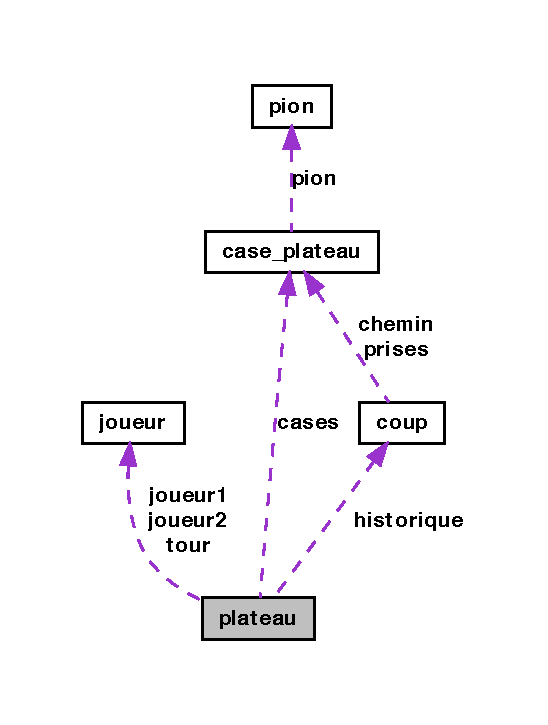
\includegraphics[width=263pt]{structplateau__coll__graph}
\end{center}
\end{figure}
\subsection*{Champs de données}
\begin{DoxyCompactItemize}
\item 
\hyperlink{structcase__plateau}{case\_\-plateau} \hyperlink{structplateau_a6afaa60f594542e0d742b0c6d3223392}{cases} \mbox{[}51\mbox{]}
\item 
\hyperlink{structcoup}{coup} \hyperlink{structplateau_acc4d709134322b5c07f99ea2efd053ef}{historique} \mbox{[}500\mbox{]}
\item 
int \hyperlink{structplateau_acb559820d9ca11295b4500f179ef6392}{i}
\item 
\hypertarget{structplateau_a82980352d73c284ef3e383cd6d264684}{
\hyperlink{structjoueur}{joueur} {\bfseries joueur1}}
\label{structplateau_a82980352d73c284ef3e383cd6d264684}

\item 
\hypertarget{structplateau_ae69884370ccd25538fe0885e68dc6c76}{
\hyperlink{structjoueur}{joueur} {\bfseries joueur2}}
\label{structplateau_ae69884370ccd25538fe0885e68dc6c76}

\item 
\hyperlink{structjoueur}{joueur} \hyperlink{structplateau_ab38c06b0c7e61b9eeb63b04c5e5bc652}{tour}
\end{DoxyCompactItemize}


\subsection{Description détaillée}
Objet plateau. Le plateau est composé de 50 cases, numérotées de 1 à 50. Il comporte un historique des coups. Il sait quel joueur doit jouer le prochain coup. 

Définition à la ligne \hyperlink{plateau_8h_source_l00107}{107} du fichier \hyperlink{plateau_8h_source}{plateau.h}.



\subsection{Documentation des champs}
\hypertarget{structplateau_a6afaa60f594542e0d742b0c6d3223392}{
\index{plateau@{plateau}!cases@{cases}}
\index{cases@{cases}!plateau@{plateau}}
\subsubsection[{cases}]{\setlength{\rightskip}{0pt plus 5cm}{\bf case\_\-plateau} {\bf cases}\mbox{[}51\mbox{]}}}
\label{structplateau_a6afaa60f594542e0d742b0c6d3223392}
Un plateau est composé de 50 cases, numérotées de 01 à 50. (la case 0 stocke la case blanche). 

Définition à la ligne \hyperlink{plateau_8h_source_l00108}{108} du fichier \hyperlink{plateau_8h_source}{plateau.h}.

\hypertarget{structplateau_acc4d709134322b5c07f99ea2efd053ef}{
\index{plateau@{plateau}!historique@{historique}}
\index{historique@{historique}!plateau@{plateau}}
\subsubsection[{historique}]{\setlength{\rightskip}{0pt plus 5cm}{\bf coup} {\bf historique}\mbox{[}500\mbox{]}}}
\label{structplateau_acc4d709134322b5c07f99ea2efd053ef}
On peut enregistrer jusqu'à 500 coups. 

Définition à la ligne \hyperlink{plateau_8h_source_l00109}{109} du fichier \hyperlink{plateau_8h_source}{plateau.h}.

\hypertarget{structplateau_acb559820d9ca11295b4500f179ef6392}{
\index{plateau@{plateau}!i@{i}}
\index{i@{i}!plateau@{plateau}}
\subsubsection[{i}]{\setlength{\rightskip}{0pt plus 5cm}int {\bf i}}}
\label{structplateau_acb559820d9ca11295b4500f179ef6392}
Non utilisé : l'indice du prochain coup à entrer. 

Définition à la ligne \hyperlink{plateau_8h_source_l00110}{110} du fichier \hyperlink{plateau_8h_source}{plateau.h}.

\hypertarget{structplateau_ab38c06b0c7e61b9eeb63b04c5e5bc652}{
\index{plateau@{plateau}!tour@{tour}}
\index{tour@{tour}!plateau@{plateau}}
\subsubsection[{tour}]{\setlength{\rightskip}{0pt plus 5cm}{\bf joueur} {\bf tour}}}
\label{structplateau_ab38c06b0c7e61b9eeb63b04c5e5bc652}
Le joueur qui doit jouer le prochain coup. 

Définition à la ligne \hyperlink{plateau_8h_source_l00113}{113} du fichier \hyperlink{plateau_8h_source}{plateau.h}.



La documentation de cette structure a été générée à partir du fichier suivant :\begin{DoxyCompactItemize}
\item 
\hyperlink{plateau_8h}{plateau.h}\end{DoxyCompactItemize}

\chapter{Documentation des fichiers}
\hypertarget{arbre_8h}{
\section{Référence du fichier arbre.h}
\label{arbre_8h}\index{arbre.h@{arbre.h}}
}


Implémantation des arbres.  


Ce graphe montre quels fichiers incluent directement ou indirectement ce fichier :
\nopagebreak
\begin{figure}[H]
\begin{center}
\leavevmode
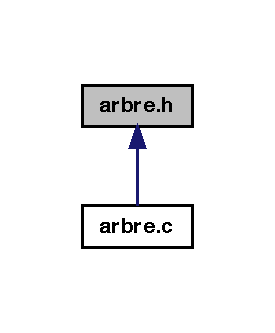
\includegraphics[width=132pt]{arbre_8h__dep__incl}
\end{center}
\end{figure}
\subsection*{Structures de données}
\begin{DoxyCompactItemize}
\item 
struct \hyperlink{structarbre}{arbre}
\begin{DoxyCompactList}\small\item\em Un arbre à une valeur (la racine) et un certain nombre de fils. \item\end{DoxyCompactList}\end{DoxyCompactItemize}
\subsection*{Définition de type}
\begin{DoxyCompactItemize}
\item 
\hypertarget{arbre_8h_adc50a5473fc43e43d9591a8ff5e3fa5c}{
typedef struct \hyperlink{structarbre}{arbre} {\bfseries arbre}}
\label{arbre_8h_adc50a5473fc43e43d9591a8ff5e3fa5c}

\end{DoxyCompactItemize}
\subsection*{Fonctions}
\begin{DoxyCompactItemize}
\item 
\hypertarget{arbre_8h_aa76e6b4b8f176cc99eb68cd16ed968a6}{
int \hyperlink{arbre_8h_aa76e6b4b8f176cc99eb68cd16ed968a6}{arbre\_\-est\_\-feuille} (\hyperlink{structarbre}{arbre} t)}
\label{arbre_8h_aa76e6b4b8f176cc99eb68cd16ed968a6}

\begin{DoxyCompactList}\small\item\em Renvoie vrai si l'arbre est une feuille. \item\end{DoxyCompactList}\item 
\hypertarget{arbre_8h_a3ee0f190b2bd5e4f94d53c3ad6730c52}{
void \hyperlink{arbre_8h_a3ee0f190b2bd5e4f94d53c3ad6730c52}{print\_\-arbre} (\hyperlink{structarbre}{arbre} t)}
\label{arbre_8h_a3ee0f190b2bd5e4f94d53c3ad6730c52}

\begin{DoxyCompactList}\small\item\em Affiche l'arbre en parcours préfixe \char`\"{}à la Scheme\char`\"{}, c.à.d. de la forme (racine fils1 fils2 ...). \item\end{DoxyCompactList}\end{DoxyCompactItemize}


\subsection{Description détaillée}
Implémantation des arbres. \begin{DoxyAuthor}{Auteur}
Bastien Auda 
\end{DoxyAuthor}


Définition dans le fichier \hyperlink{arbre_8h_source}{arbre.h}.


\hypertarget{arbre_8h_source}{
\section{arbre.h}
}

\begin{DoxyCode}
00001 
\hypertarget{arbre_8h_source_l00013}{}\hyperlink{structarbre}{00013} \textcolor{keyword}{typedef} \textcolor{keyword}{struct }\hyperlink{structarbre}{arbre} \{
00014         \textcolor{keyword}{struct }\hyperlink{structarbre}{arbre} * parent;
00015         \textcolor{keywordtype}{int} valeur;
00016         \textcolor{keywordtype}{int} profondeur;
\hypertarget{arbre_8h_source_l00017}{}\hyperlink{structarbre_a67c44f020d501282adc38e3301a5f245}{00017}         \textcolor{keywordtype}{int} \hyperlink{structarbre_a67c44f020d501282adc38e3301a5f245}{nb_fils}; 
\hypertarget{arbre_8h_source_l00018}{}\hyperlink{structarbre_a7bac08e3c2aedbde0dddf80b94eadf76}{00018}         \textcolor{keyword}{struct }\hyperlink{structarbre}{arbre} *\hyperlink{structarbre_a7bac08e3c2aedbde0dddf80b94eadf76}{fils}[80]; 
00019 \} \hyperlink{structarbre}{arbre};
00020 
00021 
00026 \textcolor{keywordtype}{int} arbre\_est\_feuille(\hyperlink{structarbre}{arbre} \hyperlink{plateau_8h_a9e00f85b4b6ec2d8bdfbe94ff40f0eeea0247320c476fffeaa81ffa7836e08dee}{t});
00027 
00032 \textcolor{keywordtype}{void} print\_arbre(\hyperlink{structarbre}{arbre} \hyperlink{plateau_8h_a9e00f85b4b6ec2d8bdfbe94ff40f0eeea0247320c476fffeaa81ffa7836e08dee}{t});
\end{DoxyCode}

\hypertarget{constantes_8h}{
\section{Référence du fichier constantes.h}
\label{constantes_8h}\index{constantes.h@{constantes.h}}
}


Constantes utiles pour l'interface.  


Ce graphe montre quels fichiers incluent directement ou indirectement ce fichier :
\nopagebreak
\begin{figure}[H]
\begin{center}
\leavevmode
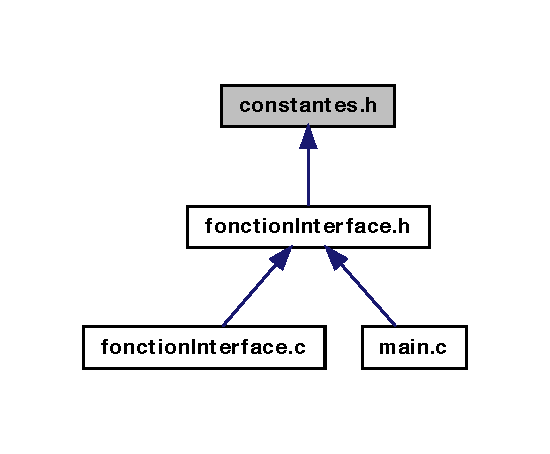
\includegraphics[width=264pt]{constantes_8h__dep__incl}
\end{center}
\end{figure}
\subsection*{Structures de données}
\begin{DoxyCompactItemize}
\item 
struct \hyperlink{struct_carre__fonce}{Carre\_\-fonce}
\item 
struct \hyperlink{struct_carre__clair}{Carre\_\-clair}
\item 
struct \hyperlink{struct_pion__clair}{Pion\_\-clair}
\item 
struct \hyperlink{struct_pion__fonce}{Pion\_\-fonce}
\end{DoxyCompactItemize}
\subsection*{Macros}
\begin{DoxyCompactItemize}
\item 
\hypertarget{constantes_8h_a4ca172d6f0e02723bb525753ccc5b2ba}{
\#define {\bfseries CONSTANTES\_\-H\_\-}}
\label{constantes_8h_a4ca172d6f0e02723bb525753ccc5b2ba}

\item 
\hypertarget{constantes_8h_a3d3bf5a2f88b1dba6c6bc13bf889c3cc}{
\#define {\bfseries LARGEUR}~800}
\label{constantes_8h_a3d3bf5a2f88b1dba6c6bc13bf889c3cc}

\item 
\hypertarget{constantes_8h_aa1d59e1f29f3ef8e058867d3e5c0b694}{
\#define {\bfseries LONGUEUR}~800}
\label{constantes_8h_aa1d59e1f29f3ef8e058867d3e5c0b694}

\item 
\hypertarget{constantes_8h_a296a42b3825f6143319944bac2b50ddb}{
\#define {\bfseries TAILLECARRE}~80}
\label{constantes_8h_a296a42b3825f6143319944bac2b50ddb}

\end{DoxyCompactItemize}


\subsection{Description détaillée}
Constantes utiles pour l'interface. \begin{DoxyAuthor}{Auteur}
Mrah Mehdi 
\end{DoxyAuthor}


Définition dans le fichier \hyperlink{constantes_8h_source}{constantes.h}.


\hypertarget{constantes_8h_source}{
\section{constantes.h}
}

\begin{DoxyCode}
00001 
00009 \textcolor{preprocessor}{#if defined(linux) || defined(\_\_linux) || defined(\_\_linux\_\_)}
00010 \textcolor{preprocessor}{}\textcolor{preprocessor}{#include <SDL/SDL.h>}
00011 \textcolor{preprocessor}{#endif}
00012 \textcolor{preprocessor}{}\textcolor{preprocessor}{#if defined(\_\_APPLE\_\_)}
00013 \textcolor{preprocessor}{}\textcolor{preprocessor}{#include <SDL/SDL.h>}
00014 \textcolor{preprocessor}{#endif}
00015 \textcolor{preprocessor}{}\textcolor{preprocessor}{#if defined(WIN32) || defined(\_WIN32) || defined(WIN64) || defined(\_WIN64)}
00016 \textcolor{preprocessor}{}\textcolor{preprocessor}{#include <SDL\(\backslash\)SDL.h>}
00017 \textcolor{preprocessor}{#endif}
00018 \textcolor{preprocessor}{}
00019 
00020 \textcolor{preprocessor}{#ifndef CONSTANTES\_H\_}
00021 \textcolor{preprocessor}{}\textcolor{preprocessor}{#define CONSTANTES\_H\_}
00022 \textcolor{preprocessor}{}
00023 
00024 \textcolor{preprocessor}{#define LARGEUR 800}
00025 \textcolor{preprocessor}{}\textcolor{preprocessor}{#define LONGUEUR 800}
00026 \textcolor{preprocessor}{}\textcolor{preprocessor}{#define TAILLECARRE 80}
00027 \textcolor{preprocessor}{}
\hypertarget{constantes_8h_source_l00029}{}\hyperlink{struct_carre__fonce}{00029} \textcolor{keyword}{typedef} \textcolor{keyword}{struct }\{
00030         \textcolor{keywordtype}{int} est\_libre;
00031         \textcolor{keywordtype}{int} numero\_case;
00032         SDL\_Rect position;
00033         SDL\_Surface *surface;
00034 \} \hyperlink{struct_carre__fonce}{Carre_fonce};
00035 
\hypertarget{constantes_8h_source_l00037}{}\hyperlink{struct_carre__clair}{00037} \textcolor{keyword}{typedef} \textcolor{keyword}{struct }\{
00038         \textcolor{keywordtype}{int} est\_libre;
00039         \textcolor{keywordtype}{int} numero\_case;
00040         SDL\_Rect position;
00041         SDL\_Surface *surface;
00042 \} \hyperlink{struct_carre__clair}{Carre_clair};
00043 
\hypertarget{constantes_8h_source_l00045}{}\hyperlink{struct_pion__clair}{00045} \textcolor{keyword}{typedef} \textcolor{keyword}{struct}\{
00046         \textcolor{keywordtype}{int} est\_dame;
00047         SDL\_Surface *surface;
00048         SDL\_Rect position;
00049 \} \hyperlink{struct_pion__clair}{Pion_clair};
00050 
\hypertarget{constantes_8h_source_l00052}{}\hyperlink{struct_pion__fonce}{00052} \textcolor{keyword}{typedef} \textcolor{keyword}{struct}\{
00053         \textcolor{keywordtype}{int} est\_dame;
00054         SDL\_Surface *surface;
00055         SDL\_Rect position;
00056 \} \hyperlink{struct_pion__fonce}{Pion_fonce};
00057 
00058 \textcolor{preprocessor}{#endif}
\end{DoxyCode}

\hypertarget{fonction__evaluation_8h}{
\section{Référence du fichier fonction\_\-evaluation.h}
\label{fonction__evaluation_8h}\index{fonction\_\-evaluation.h@{fonction\_\-evaluation.h}}
}


La fonction d'evaluation de l'algorithme MinMax. Renvoie un double compris entre -\/1 et 1 caracterisant un etat du plateau plus ou moins favorable au joueur courant.  


{\ttfamily \#include $<$stdio.h$>$}\par
{\ttfamily \#include $<$stdlib.h$>$}\par
{\ttfamily \#include \char`\"{}regles.h\char`\"{}}\par
Graphe des dépendances par inclusion de fonction\_\-evaluation.h:\nopagebreak
\begin{figure}[H]
\begin{center}
\leavevmode
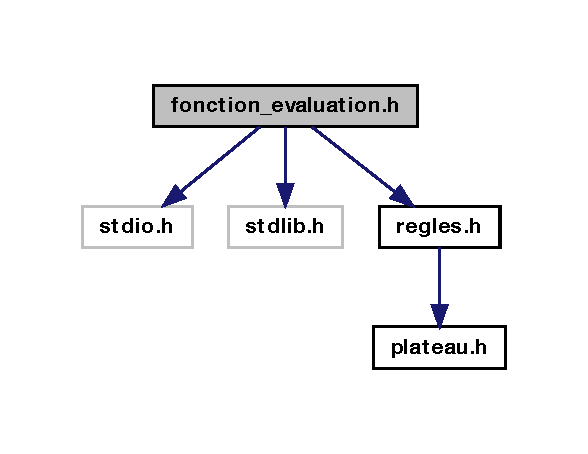
\includegraphics[width=282pt]{fonction__evaluation_8h__incl}
\end{center}
\end{figure}
Ce graphe montre quels fichiers incluent directement ou indirectement ce fichier :
\nopagebreak
\begin{figure}[H]
\begin{center}
\leavevmode
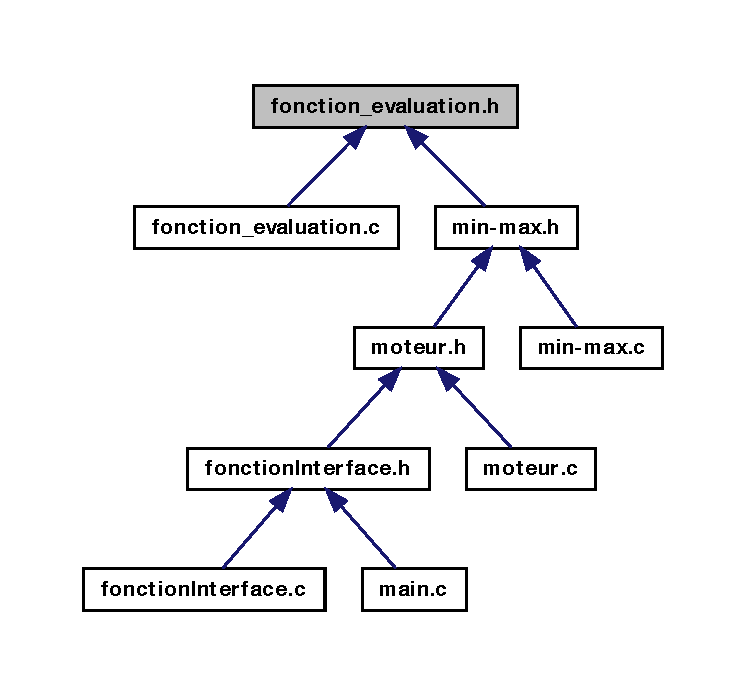
\includegraphics[width=358pt]{fonction__evaluation_8h__dep__incl}
\end{center}
\end{figure}
\subsection*{Fonctions}
\begin{DoxyCompactItemize}
\item 
\hypertarget{fonction__evaluation_8h_a0c58a26787b1d2de66cf1304ce4b9b7d}{
double {\bfseries fct\_\-eval} (const \hyperlink{structplateau}{plateau} $\ast$p)}
\label{fonction__evaluation_8h_a0c58a26787b1d2de66cf1304ce4b9b7d}

\item 
\hypertarget{fonction__evaluation_8h_a5a3806fc0e2c63b27df150e5534f4ba7}{
int {\bfseries valeur\_\-case} (const \hyperlink{structplateau}{plateau} $\ast$p, const \hyperlink{structcase__plateau}{case\_\-plateau} $\ast$c)}
\label{fonction__evaluation_8h_a5a3806fc0e2c63b27df150e5534f4ba7}

\item 
\hypertarget{fonction__evaluation_8h_af8b5f84ce8e389aa6afa02c33871c69d}{
int \hyperlink{fonction__evaluation_8h_af8b5f84ce8e389aa6afa02c33871c69d}{rang} (const \hyperlink{structcase__plateau}{case\_\-plateau} $\ast$c)}
\label{fonction__evaluation_8h_af8b5f84ce8e389aa6afa02c33871c69d}

\begin{DoxyCompactList}\small\item\em Renvoie, pour une case occupee, son rang ie le numero de sa ligne. (depend du camp du pion) \item\end{DoxyCompactList}\item 
\hypertarget{fonction__evaluation_8h_ad2e3a41e13c24a4f05dde2144f7a9124}{
int \hyperlink{fonction__evaluation_8h_ad2e3a41e13c24a4f05dde2144f7a9124}{est\_\-isole} (const \hyperlink{structplateau}{plateau} $\ast$p, const \hyperlink{structcase__plateau}{case\_\-plateau} $\ast$c, int rang)}
\label{fonction__evaluation_8h_ad2e3a41e13c24a4f05dde2144f7a9124}

\begin{DoxyCompactList}\small\item\em un pion isole n'est pas sur un bord et n'a aucun pion de son camp present dans une case adjacente. \item\end{DoxyCompactList}\end{DoxyCompactItemize}


\subsection{Description détaillée}
La fonction d'evaluation de l'algorithme MinMax. Renvoie un double compris entre -\/1 et 1 caracterisant un etat du plateau plus ou moins favorable au joueur courant. \begin{DoxyAuthor}{Auteur}
Kyann Valai 
\end{DoxyAuthor}


Définition dans le fichier \hyperlink{fonction__evaluation_8h_source}{fonction\_\-evaluation.h}.


\hypertarget{fonction__evaluation_8h_source}{
\section{fonction\_\-evaluation.h}
}

\begin{DoxyCode}
00001 
00008 \textcolor{preprocessor}{#include <stdio.h>}
00009 \textcolor{preprocessor}{#include <stdlib.h>}
00010 \textcolor{preprocessor}{#include "\hyperlink{regles_8h}{regles.h}"}
00011 
00018 \textcolor{keywordtype}{double} fct\_eval(\textcolor{keyword}{const} \hyperlink{structplateau}{plateau} * p);
00019 
00024 \textcolor{keywordtype}{int} valeur\_case(\textcolor{keyword}{const} \hyperlink{structplateau}{plateau} * p, \textcolor{keyword}{const} \hyperlink{structcase__plateau}{case_plateau} * c);
00025 
00030 \textcolor{keywordtype}{int} rang(\textcolor{keyword}{const} \hyperlink{structcase__plateau}{case_plateau} * c);
00031 
00036 \textcolor{keywordtype}{int} est\_isole(\textcolor{keyword}{const} \hyperlink{structplateau}{plateau} * p, \textcolor{keyword}{const} \hyperlink{structcase__plateau}{case_plateau} * c, \textcolor{keywordtype}{int} rang);
\end{DoxyCode}

\hypertarget{fonction_interface_8h}{
\section{Référence du fichier fonctionInterface.h}
\label{fonction_interface_8h}\index{fonctionInterface.h@{fonctionInterface.h}}
}


Implémentation de fonctionnalités pour l'interface.  


{\ttfamily \#include \char`\"{}constantes.h\char`\"{}}\par
{\ttfamily \#include \char`\"{}moteur.h\char`\"{}}\par
Graphe des dépendances par inclusion de fonctionInterface.h:\nopagebreak
\begin{figure}[H]
\begin{center}
\leavevmode
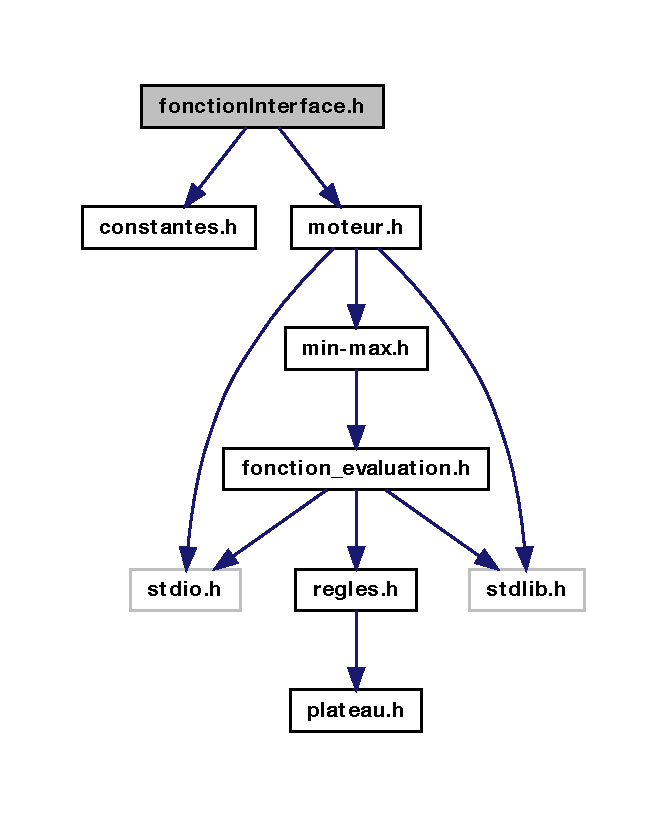
\includegraphics[width=320pt]{fonction_interface_8h__incl}
\end{center}
\end{figure}
Ce graphe montre quels fichiers incluent directement ou indirectement ce fichier :
\nopagebreak
\begin{figure}[H]
\begin{center}
\leavevmode
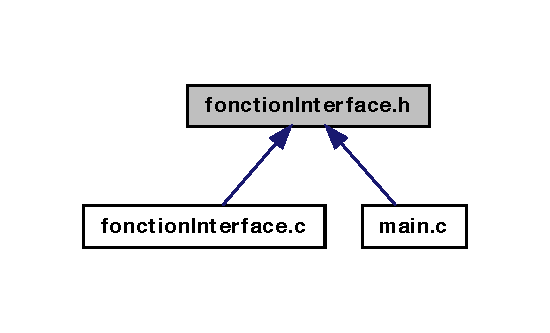
\includegraphics[width=264pt]{fonction_interface_8h__dep__incl}
\end{center}
\end{figure}
\subsection*{Fonctions}
\begin{DoxyCompactItemize}
\item 
\hypertarget{fonction_interface_8h_a242025f62105b1932bde128f77ec1ba8}{
void \hyperlink{fonction_interface_8h_a242025f62105b1932bde128f77ec1ba8}{rafraichir\_\-plateau} ()}
\label{fonction_interface_8h_a242025f62105b1932bde128f77ec1ba8}

\begin{DoxyCompactList}\small\item\em Rafraichit le plateau aprés une action. \item\end{DoxyCompactList}\item 
void \hyperlink{fonction_interface_8h_afea6e76f6f28549c9c1f44636d93cb82}{afficher\_\-ecran\_\-depart\_\-neutre} (int choix)
\begin{DoxyCompactList}\small\item\em Affiche le menu de depart. \item\end{DoxyCompactList}\item 
\hypertarget{fonction_interface_8h_a1cbeb954df481f599bb888cda252b37c}{
void {\bfseries afficher\_\-ecran\_\-pause} (int choix)}
\label{fonction_interface_8h_a1cbeb954df481f599bb888cda252b37c}

\item 
\hypertarget{fonction_interface_8h_a57441c18ac94ad4618d8ecd732b8ec2b}{
void \hyperlink{fonction_interface_8h_a57441c18ac94ad4618d8ecd732b8ec2b}{afficher\_\-ecran\_\-choix\_\-joueur} ()}
\label{fonction_interface_8h_a57441c18ac94ad4618d8ecd732b8ec2b}

\begin{DoxyCompactList}\small\item\em Affiche le menu de choix IA/Joueur. \item\end{DoxyCompactList}\item 
\hypertarget{fonction_interface_8h_a4eaec2179ee4e6fc89c1c06b74e94cb4}{
void \hyperlink{fonction_interface_8h_a4eaec2179ee4e6fc89c1c06b74e94cb4}{afficher\_\-ecran\_\-noirs\_\-gagnent} ()}
\label{fonction_interface_8h_a4eaec2179ee4e6fc89c1c06b74e94cb4}

\begin{DoxyCompactList}\small\item\em Affiche l'ecran de fin de partie, les noirs gagnent. \item\end{DoxyCompactList}\item 
\hypertarget{fonction_interface_8h_acc462fb032b8caf056324a003ae36497}{
void \hyperlink{fonction_interface_8h_acc462fb032b8caf056324a003ae36497}{afficher\_\-ecran\_\-blancs\_\-gagnent} ()}
\label{fonction_interface_8h_acc462fb032b8caf056324a003ae36497}

\begin{DoxyCompactList}\small\item\em Affiche l'ecran de fin de partie, les blancs gagnent. \item\end{DoxyCompactList}\item 
int \hyperlink{fonction_interface_8h_af439094b4dbb8cac323aaba6130a3cfb}{clique\_\-souris\_\-choix\_\-joueur} (SDL\_\-Event evenement)
\begin{DoxyCompactList}\small\item\em Retourne la position de la souris après un clique dans le menu choix IA/Joueur. \item\end{DoxyCompactList}\item 
int $\ast$ \hyperlink{fonction_interface_8h_af90df7e39dda6c350185ce94e31fb93c}{clique\_\-souris} (SDL\_\-Event evenement)
\begin{DoxyCompactList}\small\item\em Retourne la position de la souris après un clique. \item\end{DoxyCompactList}\item 
\hypertarget{fonction_interface_8h_a757ae0e029a9f8857391b1fb5939d54a}{
void \hyperlink{fonction_interface_8h_a757ae0e029a9f8857391b1fb5939d54a}{initialisation\_\-cases\_\-blanches} ()}
\label{fonction_interface_8h_a757ae0e029a9f8857391b1fb5939d54a}

\begin{DoxyCompactList}\small\item\em Initialise les cases blanches. \item\end{DoxyCompactList}\item 
int \hyperlink{fonction_interface_8h_a22f816def98b98aae351ce6087c763ef}{position\_\-souris} (SDL\_\-Event evenement)
\begin{DoxyCompactList}\small\item\em Calcule la position de la souris a chaque mouvement. \item\end{DoxyCompactList}\item 
\hypertarget{fonction_interface_8h_a76c5afeb8abd24f73406af4dbeaa3b73}{
int {\bfseries position\_\-souris\_\-pause} (SDL\_\-Event evenement)}
\label{fonction_interface_8h_a76c5afeb8abd24f73406af4dbeaa3b73}

\item 
\hypertarget{fonction_interface_8h_a00d8cde866b4a76fff71b46e24e5ea4f}{
int {\bfseries clique\_\-souris\_\-menu} (SDL\_\-Event evenement)}
\label{fonction_interface_8h_a00d8cde866b4a76fff71b46e24e5ea4f}

\item 
\hypertarget{fonction_interface_8h_a5f8c294b42841b329969d4fc823c9d07}{
int {\bfseries clique\_\-souris\_\-pause} (SDL\_\-Event evenement)}
\label{fonction_interface_8h_a5f8c294b42841b329969d4fc823c9d07}

\item 
\hypertarget{fonction_interface_8h_a1207c39d2959b1cf52223c10bee518a7}{
void {\bfseries control\_\-manger\_\-pion} (\hyperlink{structcase__plateau}{case\_\-plateau} oldPosition, \hyperlink{structcase__plateau}{case\_\-plateau} newPosition)}
\label{fonction_interface_8h_a1207c39d2959b1cf52223c10bee518a7}

\item 
\hypertarget{fonction_interface_8h_a2d99a85898da4d9f5578a1ec59fc0db1}{
\hyperlink{structcase__plateau}{case\_\-plateau} {\bfseries control\_\-surbrillance} (int $\ast$tab)}
\label{fonction_interface_8h_a2d99a85898da4d9f5578a1ec59fc0db1}

\item 
\hyperlink{structcase__plateau}{case\_\-plateau} \hyperlink{fonction_interface_8h_abcb8707f8b1169dceb38a3e3e2b3e300}{control\_\-premier\_\-click} (SDL\_\-Event event, int $\ast$tab, \hyperlink{structplateau}{plateau} $\ast$p, \hyperlink{structcase__plateau}{case\_\-plateau} $\ast$oldCase)
\begin{DoxyCompactList}\small\item\em Gere le premier click qui s'occupe uniquement de la selection du pion a jouer. \item\end{DoxyCompactList}\item 
\hypertarget{fonction_interface_8h_acb796f12694cf5cfa8b3ecddfdf3619b}{
\hyperlink{structcase__plateau}{case\_\-plateau} {\bfseries control\_\-deuxieme\_\-click} (SDL\_\-Event event, int $\ast$tab, \hyperlink{structplateau}{plateau} $\ast$p, \hyperlink{structcase__plateau}{case\_\-plateau} $\ast$newCase, \hyperlink{structcase__plateau}{case\_\-plateau} $\ast$oldCase)}
\label{fonction_interface_8h_acb796f12694cf5cfa8b3ecddfdf3619b}

\end{DoxyCompactItemize}
\subsection*{Variables}
\begin{DoxyCompactItemize}
\item 
\hyperlink{struct_carre__fonce}{Carre\_\-fonce} \hyperlink{fonction_interface_8h_a7e67ffd6431a872b2e0eed3293230b78}{carre\_\-fonce}
\item 
\hyperlink{struct_carre__clair}{Carre\_\-clair} \hyperlink{fonction_interface_8h_aa6a56f4dc2396c5f9de42147f569c367}{carre\_\-clair}
\item 
\hyperlink{struct_carre__clair}{Carre\_\-clair} \hyperlink{fonction_interface_8h_a28e2678f1d8d143ee4b21a11acfad35d}{carre\_\-surbrillance}
\item 
\hyperlink{struct_pion__clair}{Pion\_\-clair} \hyperlink{fonction_interface_8h_ae7267ac64141d082948941a1b51d4df6}{pion\_\-clair}
\item 
\hyperlink{struct_pion__fonce}{Pion\_\-fonce} \hyperlink{fonction_interface_8h_a91d0d5668d6c4d2c6cd5bbeab0f9ca15}{pion\_\-fonce}
\item 
SDL\_\-Surface $\ast$ \hyperlink{fonction_interface_8h_a78fa3957d73de49cb81d047857504218}{screen}
\item 
\hypertarget{fonction_interface_8h_a7352e9ae5b20378e23568a8a6ddcf0e2}{
int {\bfseries tableauChoix} \mbox{[}4\mbox{]}}
\label{fonction_interface_8h_a7352e9ae5b20378e23568a8a6ddcf0e2}

\end{DoxyCompactItemize}


\subsection{Description détaillée}
Implémentation de fonctionnalités pour l'interface. \begin{DoxyAuthor}{Auteur}
Mrah Mehdi 
\end{DoxyAuthor}


Définition dans le fichier \hyperlink{fonction_interface_8h_source}{fonctionInterface.h}.



\subsection{Documentation des fonctions}
\hypertarget{fonction_interface_8h_afea6e76f6f28549c9c1f44636d93cb82}{
\index{fonctionInterface.h@{fonctionInterface.h}!afficher\_\-ecran\_\-depart\_\-neutre@{afficher\_\-ecran\_\-depart\_\-neutre}}
\index{afficher\_\-ecran\_\-depart\_\-neutre@{afficher\_\-ecran\_\-depart\_\-neutre}!fonctionInterface.h@{fonctionInterface.h}}
\subsubsection[{afficher\_\-ecran\_\-depart\_\-neutre}]{\setlength{\rightskip}{0pt plus 5cm}void afficher\_\-ecran\_\-depart\_\-neutre (
\begin{DoxyParamCaption}
\item[{int}]{choix}
\end{DoxyParamCaption}
)}}
\label{fonction_interface_8h_afea6e76f6f28549c9c1f44636d93cb82}


Affiche le menu de depart. 

Affiche le menu pause.


\begin{DoxyParams}{Paramètres}
{\em choix} & Represente le choix dans le menu depart.\\
\hline
{\em choix} & Represente le choix dans le menu pause. \\
\hline
\end{DoxyParams}


Définition à la ligne \hyperlink{fonction_interface_8c_source_l00118}{118} du fichier \hyperlink{fonction_interface_8c_source}{fonctionInterface.c}.

\hypertarget{fonction_interface_8h_af90df7e39dda6c350185ce94e31fb93c}{
\index{fonctionInterface.h@{fonctionInterface.h}!clique\_\-souris@{clique\_\-souris}}
\index{clique\_\-souris@{clique\_\-souris}!fonctionInterface.h@{fonctionInterface.h}}
\subsubsection[{clique\_\-souris}]{\setlength{\rightskip}{0pt plus 5cm}int$\ast$ clique\_\-souris (
\begin{DoxyParamCaption}
\item[{SDL\_\-Event}]{evenement}
\end{DoxyParamCaption}
)}}
\label{fonction_interface_8h_af90df7e39dda6c350185ce94e31fb93c}


Retourne la position de la souris après un clique. 

\begin{DoxyReturn}{Renvoie}
int$\ast$ Un tableau contenant la position x et y du clique 
\end{DoxyReturn}


Définition à la ligne \hyperlink{fonction_interface_8c_source_l00263}{263} du fichier \hyperlink{fonction_interface_8c_source}{fonctionInterface.c}.

\hypertarget{fonction_interface_8h_af439094b4dbb8cac323aaba6130a3cfb}{
\index{fonctionInterface.h@{fonctionInterface.h}!clique\_\-souris\_\-choix\_\-joueur@{clique\_\-souris\_\-choix\_\-joueur}}
\index{clique\_\-souris\_\-choix\_\-joueur@{clique\_\-souris\_\-choix\_\-joueur}!fonctionInterface.h@{fonctionInterface.h}}
\subsubsection[{clique\_\-souris\_\-choix\_\-joueur}]{\setlength{\rightskip}{0pt plus 5cm}int clique\_\-souris\_\-choix\_\-joueur (
\begin{DoxyParamCaption}
\item[{SDL\_\-Event}]{evenement}
\end{DoxyParamCaption}
)}}
\label{fonction_interface_8h_af439094b4dbb8cac323aaba6130a3cfb}


Retourne la position de la souris après un clique dans le menu choix IA/Joueur. 

\begin{DoxyReturn}{Renvoie}
int Un entier representant le choix du joueur. 
\end{DoxyReturn}


Définition à la ligne \hyperlink{fonction_interface_8c_source_l00301}{301} du fichier \hyperlink{fonction_interface_8c_source}{fonctionInterface.c}.

\hypertarget{fonction_interface_8h_abcb8707f8b1169dceb38a3e3e2b3e300}{
\index{fonctionInterface.h@{fonctionInterface.h}!control\_\-premier\_\-click@{control\_\-premier\_\-click}}
\index{control\_\-premier\_\-click@{control\_\-premier\_\-click}!fonctionInterface.h@{fonctionInterface.h}}
\subsubsection[{control\_\-premier\_\-click}]{\setlength{\rightskip}{0pt plus 5cm}{\bf case\_\-plateau} control\_\-premier\_\-click (
\begin{DoxyParamCaption}
\item[{SDL\_\-Event}]{event, }
\item[{int $\ast$}]{tab, }
\item[{{\bf plateau} $\ast$}]{p, }
\item[{{\bf case\_\-plateau} $\ast$}]{oldCase}
\end{DoxyParamCaption}
)}}
\label{fonction_interface_8h_abcb8707f8b1169dceb38a3e3e2b3e300}


Gere le premier click qui s'occupe uniquement de la selection du pion a jouer. 


\begin{DoxyParams}{Paramètres}
{\em tab} & Tableau contenant les coordonnees du click \\
\hline
{\em oldCase} & la case de depart \\
\hline
\end{DoxyParams}
\begin{DoxyReturn}{Renvoie}
\hyperlink{structcase__plateau}{case\_\-plateau} La case contenant le pion selectionne 
\end{DoxyReturn}
\begin{DoxyAuthor}{Auteur}
Mehdi M'rah 
\end{DoxyAuthor}


Définition à la ligne \hyperlink{fonction_interface_8c_source_l00515}{515} du fichier \hyperlink{fonction_interface_8c_source}{fonctionInterface.c}.

\hypertarget{fonction_interface_8h_a22f816def98b98aae351ce6087c763ef}{
\index{fonctionInterface.h@{fonctionInterface.h}!position\_\-souris@{position\_\-souris}}
\index{position\_\-souris@{position\_\-souris}!fonctionInterface.h@{fonctionInterface.h}}
\subsubsection[{position\_\-souris}]{\setlength{\rightskip}{0pt plus 5cm}int position\_\-souris (
\begin{DoxyParamCaption}
\item[{SDL\_\-Event}]{evenement}
\end{DoxyParamCaption}
)}}
\label{fonction_interface_8h_a22f816def98b98aae351ce6087c763ef}


Calcule la position de la souris a chaque mouvement. 

Calcule la position de la souris a chaque clique dans le menu principal.

\begin{DoxyReturn}{Renvoie}
int Un entier representant une position dans le menu.

int Un entier representant une position dans le menu pause.

int Un entier representant un choix dans le menu principal.

int Un entier representant un choix dans le menu pause. 
\end{DoxyReturn}


Définition à la ligne \hyperlink{fonction_interface_8c_source_l00279}{279} du fichier \hyperlink{fonction_interface_8c_source}{fonctionInterface.c}.



\subsection{Documentation des variables}
\hypertarget{fonction_interface_8h_aa6a56f4dc2396c5f9de42147f569c367}{
\index{fonctionInterface.h@{fonctionInterface.h}!carre\_\-clair@{carre\_\-clair}}
\index{carre\_\-clair@{carre\_\-clair}!fonctionInterface.h@{fonctionInterface.h}}
\subsubsection[{carre\_\-clair}]{\setlength{\rightskip}{0pt plus 5cm}{\bf Carre\_\-clair} {\bf carre\_\-clair}}}
\label{fonction_interface_8h_aa6a56f4dc2396c5f9de42147f569c367}
Surface : marbre blanc 

Définition à la ligne \hyperlink{fonction_interface_8h_source_l00019}{19} du fichier \hyperlink{fonction_interface_8h_source}{fonctionInterface.h}.

\hypertarget{fonction_interface_8h_a7e67ffd6431a872b2e0eed3293230b78}{
\index{fonctionInterface.h@{fonctionInterface.h}!carre\_\-fonce@{carre\_\-fonce}}
\index{carre\_\-fonce@{carre\_\-fonce}!fonctionInterface.h@{fonctionInterface.h}}
\subsubsection[{carre\_\-fonce}]{\setlength{\rightskip}{0pt plus 5cm}{\bf Carre\_\-fonce} {\bf carre\_\-fonce}}}
\label{fonction_interface_8h_a7e67ffd6431a872b2e0eed3293230b78}
Surface : marbre noir 

Définition à la ligne \hyperlink{fonction_interface_8h_source_l00016}{16} du fichier \hyperlink{fonction_interface_8h_source}{fonctionInterface.h}.

\hypertarget{fonction_interface_8h_a28e2678f1d8d143ee4b21a11acfad35d}{
\index{fonctionInterface.h@{fonctionInterface.h}!carre\_\-surbrillance@{carre\_\-surbrillance}}
\index{carre\_\-surbrillance@{carre\_\-surbrillance}!fonctionInterface.h@{fonctionInterface.h}}
\subsubsection[{carre\_\-surbrillance}]{\setlength{\rightskip}{0pt plus 5cm}{\bf Carre\_\-clair} {\bf carre\_\-surbrillance}}}
\label{fonction_interface_8h_a28e2678f1d8d143ee4b21a11acfad35d}
Surface : marbre noir en surbrillance 

Définition à la ligne \hyperlink{fonction_interface_8h_source_l00022}{22} du fichier \hyperlink{fonction_interface_8h_source}{fonctionInterface.h}.

\hypertarget{fonction_interface_8h_ae7267ac64141d082948941a1b51d4df6}{
\index{fonctionInterface.h@{fonctionInterface.h}!pion\_\-clair@{pion\_\-clair}}
\index{pion\_\-clair@{pion\_\-clair}!fonctionInterface.h@{fonctionInterface.h}}
\subsubsection[{pion\_\-clair}]{\setlength{\rightskip}{0pt plus 5cm}{\bf Pion\_\-clair} {\bf pion\_\-clair}}}
\label{fonction_interface_8h_ae7267ac64141d082948941a1b51d4df6}
Pion : blanc 

Définition à la ligne \hyperlink{fonction_interface_8h_source_l00025}{25} du fichier \hyperlink{fonction_interface_8h_source}{fonctionInterface.h}.

\hypertarget{fonction_interface_8h_a91d0d5668d6c4d2c6cd5bbeab0f9ca15}{
\index{fonctionInterface.h@{fonctionInterface.h}!pion\_\-fonce@{pion\_\-fonce}}
\index{pion\_\-fonce@{pion\_\-fonce}!fonctionInterface.h@{fonctionInterface.h}}
\subsubsection[{pion\_\-fonce}]{\setlength{\rightskip}{0pt plus 5cm}{\bf Pion\_\-fonce} {\bf pion\_\-fonce}}}
\label{fonction_interface_8h_a91d0d5668d6c4d2c6cd5bbeab0f9ca15}
Pion : noir 

Définition à la ligne \hyperlink{fonction_interface_8h_source_l00028}{28} du fichier \hyperlink{fonction_interface_8h_source}{fonctionInterface.h}.

\hypertarget{fonction_interface_8h_a78fa3957d73de49cb81d047857504218}{
\index{fonctionInterface.h@{fonctionInterface.h}!screen@{screen}}
\index{screen@{screen}!fonctionInterface.h@{fonctionInterface.h}}
\subsubsection[{screen}]{\setlength{\rightskip}{0pt plus 5cm}SDL\_\-Surface$\ast$ {\bf screen}}}
\label{fonction_interface_8h_a78fa3957d73de49cb81d047857504218}
Surface principal 

Définition à la ligne \hyperlink{fonction_interface_8h_source_l00031}{31} du fichier \hyperlink{fonction_interface_8h_source}{fonctionInterface.h}.


\hypertarget{fonction_interface_8h_source}{
\section{fonctionInterface.h}
}

\begin{DoxyCode}
00001 
00009 \textcolor{preprocessor}{#include "\hyperlink{constantes_8h}{constantes.h}"}
00010 \textcolor{preprocessor}{#include "\hyperlink{moteur_8h}{moteur.h}"}
00011 
00012 \textcolor{preprocessor}{#ifndef FONCTIONINTERFACE\_H\_}
00013 \textcolor{preprocessor}{}\textcolor{preprocessor}{#define FONCTIONINTERFACE\_H\_}
00014 \textcolor{preprocessor}{}
\hypertarget{fonction_interface_8h_source_l00016}{}\hyperlink{fonction_interface_8h_a7e67ffd6431a872b2e0eed3293230b78}{00016} \hyperlink{struct_carre__fonce}{Carre_fonce} \hyperlink{fonction_interface_8h_a7e67ffd6431a872b2e0eed3293230b78}{carre_fonce};
00017 
\hypertarget{fonction_interface_8h_source_l00019}{}\hyperlink{fonction_interface_8h_aa6a56f4dc2396c5f9de42147f569c367}{00019} \hyperlink{struct_carre__clair}{Carre_clair} \hyperlink{fonction_interface_8h_aa6a56f4dc2396c5f9de42147f569c367}{carre_clair};
00020 
\hypertarget{fonction_interface_8h_source_l00022}{}\hyperlink{fonction_interface_8h_a28e2678f1d8d143ee4b21a11acfad35d}{00022} \hyperlink{struct_carre__clair}{Carre_clair} \hyperlink{fonction_interface_8h_a28e2678f1d8d143ee4b21a11acfad35d}{carre_surbrillance};
00023 
\hypertarget{fonction_interface_8h_source_l00025}{}\hyperlink{fonction_interface_8h_ae7267ac64141d082948941a1b51d4df6}{00025} \hyperlink{struct_pion__clair}{Pion_clair} \hyperlink{fonction_interface_8h_ae7267ac64141d082948941a1b51d4df6}{pion_clair};
00026 
\hypertarget{fonction_interface_8h_source_l00028}{}\hyperlink{fonction_interface_8h_a91d0d5668d6c4d2c6cd5bbeab0f9ca15}{00028} \hyperlink{struct_pion__fonce}{Pion_fonce} \hyperlink{fonction_interface_8h_a91d0d5668d6c4d2c6cd5bbeab0f9ca15}{pion_fonce};
00029 
\hypertarget{fonction_interface_8h_source_l00031}{}\hyperlink{fonction_interface_8h_a78fa3957d73de49cb81d047857504218}{00031} SDL\_Surface *\hyperlink{fonction_interface_8h_a78fa3957d73de49cb81d047857504218}{screen};
00032 
00033 \textcolor{keywordtype}{int} tableauChoix[4];
00038 \textcolor{keywordtype}{void} rafraichir\_plateau();
00039 
00045 \textcolor{keywordtype}{void} afficher\_ecran\_depart\_neutre(\textcolor{keywordtype}{int} choix);
00046 
00052 \textcolor{keywordtype}{void} afficher\_ecran\_pause(\textcolor{keywordtype}{int} choix);
00053 
00058 \textcolor{keywordtype}{void} afficher\_ecran\_choix\_joueur();
00059 
00064 \textcolor{keywordtype}{void} afficher\_ecran\_noirs\_gagnent();
00065 
00070 \textcolor{keywordtype}{void} afficher\_ecran\_blancs\_gagnent();
00071 
00077 \textcolor{keywordtype}{int} clique\_souris\_choix\_joueur(SDL\_Event evenement);
00078 
00084 \textcolor{keywordtype}{int}* clique\_souris(SDL\_Event evenement);
00085 
00090 \textcolor{keywordtype}{void} initialisation\_cases\_blanches();
00091 
00097 \textcolor{keywordtype}{int} position\_souris(SDL\_Event evenement);
00103 \textcolor{keywordtype}{int} position\_souris\_pause(SDL\_Event evenement);
00109 \textcolor{keywordtype}{int} clique\_souris\_menu(SDL\_Event evenement);
00115 \textcolor{keywordtype}{int} clique\_souris\_pause(SDL\_Event evenement);
00116 
00117 
00118 \textcolor{keywordtype}{void} control\_manger\_pion(\hyperlink{structcase__plateau}{case_plateau} oldPosition, \hyperlink{structcase__plateau}{case_plateau} newPosition);
00119 
00128 \hyperlink{structcase__plateau}{case_plateau} control\_surbrillance(\textcolor{keywordtype}{int} *tab);
00129 
00138 \hyperlink{structcase__plateau}{case_plateau} control\_premier\_click(SDL\_Event event, \textcolor{keywordtype}{int} *tab, \hyperlink{structplateau}{plateau} *p, 
      \hyperlink{structcase__plateau}{case_plateau} *oldCase);
00139 
00150 \hyperlink{structcase__plateau}{case_plateau} control\_deuxieme\_click(SDL\_Event event, \textcolor{keywordtype}{int} *tab, \hyperlink{structplateau}{plateau} *p, 
      \hyperlink{structcase__plateau}{case_plateau} *newCase, \hyperlink{structcase__plateau}{case_plateau} *oldCase);
00151 
00152 \textcolor{preprocessor}{#endif }\textcolor{comment}{/* FONCTIONINTERFACE\_H\_ */}
\end{DoxyCode}

\hypertarget{min-max_8h}{
\section{Référence du fichier min-\/max.h}
\label{min-max_8h}\index{min-\/max.h@{min-\/max.h}}
}


Implémentation du min-\/max.  


{\ttfamily \#include \char`\"{}fonction\_\-evaluation.h\char`\"{}}\par
Graphe des dépendances par inclusion de min-\/max.h:\nopagebreak
\begin{figure}[H]
\begin{center}
\leavevmode
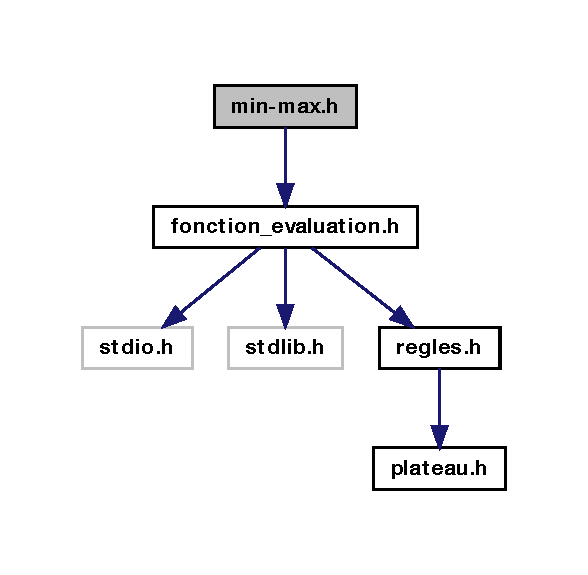
\includegraphics[width=282pt]{min-max_8h__incl}
\end{center}
\end{figure}
Ce graphe montre quels fichiers incluent directement ou indirectement ce fichier :
\nopagebreak
\begin{figure}[H]
\begin{center}
\leavevmode
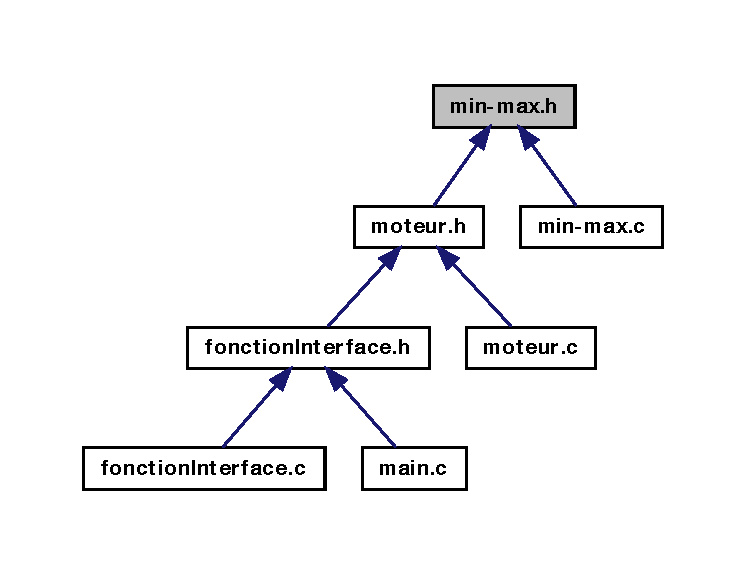
\includegraphics[width=358pt]{min-max_8h__dep__incl}
\end{center}
\end{figure}
\subsection*{Macros}
\begin{DoxyCompactItemize}
\item 
\hypertarget{min-max_8h_ab414b3d93e06e9151175e4084ed3295d}{
\#define {\bfseries MINIMUM}~-\/1}
\label{min-max_8h_ab414b3d93e06e9151175e4084ed3295d}

\item 
\hypertarget{min-max_8h_a7144aa2210e7cd9f35160cdcdaa5a648}{
\#define {\bfseries MAXIMUM}~1}
\label{min-max_8h_a7144aa2210e7cd9f35160cdcdaa5a648}

\end{DoxyCompactItemize}
\subsection*{Fonctions}
\begin{DoxyCompactItemize}
\item 
\hyperlink{structcoup}{coup} \hyperlink{min-max_8h_a5ac518ee617eb3482548c57dd2c10807}{jouerIA} (const \hyperlink{structplateau}{plateau} p, int profondeur)
\begin{DoxyCompactList}\small\item\em Renvoie le meilleur coup que peut jouer le joueur courant. \item\end{DoxyCompactList}\end{DoxyCompactItemize}


\subsection{Description détaillée}
Implémentation du min-\/max. \begin{DoxyAuthor}{Auteur}
Bastien Auda 
\end{DoxyAuthor}


Définition dans le fichier \hyperlink{min-max_8h_source}{min-\/max.h}.



\subsection{Documentation des fonctions}
\hypertarget{min-max_8h_a5ac518ee617eb3482548c57dd2c10807}{
\index{min-\/max.h@{min-\/max.h}!jouerIA@{jouerIA}}
\index{jouerIA@{jouerIA}!min-max.h@{min-\/max.h}}
\subsubsection[{jouerIA}]{\setlength{\rightskip}{0pt plus 5cm}{\bf coup} jouerIA (
\begin{DoxyParamCaption}
\item[{const {\bf plateau}}]{p, }
\item[{int}]{profondeur}
\end{DoxyParamCaption}
)}}
\label{min-max_8h_a5ac518ee617eb3482548c57dd2c10807}


Renvoie le meilleur coup que peut jouer le joueur courant. 


\begin{DoxyParams}{Paramètres}
{\em profondeur} & La profondeur à laquelle on doit utiliser la fonction d'évaluation. (profondeur $>$ 0) \\
\hline
\end{DoxyParams}


Définition à la ligne \hyperlink{min-max_8c_source_l00019}{19} du fichier \hyperlink{min-max_8c_source}{min-\/max.c}.


\hypertarget{min-max_8h_source}{
\section{min-\/max.h}
}

\begin{DoxyCode}
00001 
00009 \textcolor{preprocessor}{#define MINIMUM -1}
00010 \textcolor{preprocessor}{}\textcolor{preprocessor}{#define MAXIMUM 1}
00011 \textcolor{preprocessor}{}
00012 \textcolor{preprocessor}{#include "\hyperlink{fonction__evaluation_8h}{fonction_evaluation.h}"}
00013 
00020 \hyperlink{structcoup}{coup} jouerIA(\textcolor{keyword}{const} \hyperlink{structplateau}{plateau} p, \textcolor{keywordtype}{int} profondeur);
\end{DoxyCode}

\hypertarget{moteur_8h}{
\section{Référence du fichier moteur.h}
\label{moteur_8h}\index{moteur.h@{moteur.h}}
}


Le moteur de jeu. Il permet de gérer une partie, 1 ou 2 joueurs, fait jouer l'IA, fournit une aide au joueur.  


{\ttfamily \#include $<$stdio.h$>$}\par
{\ttfamily \#include $<$stdlib.h$>$}\par
{\ttfamily \#include \char`\"{}min-\/max.h\char`\"{}}\par
Graphe des dépendances par inclusion de moteur.h:\nopagebreak
\begin{figure}[H]
\begin{center}
\leavevmode
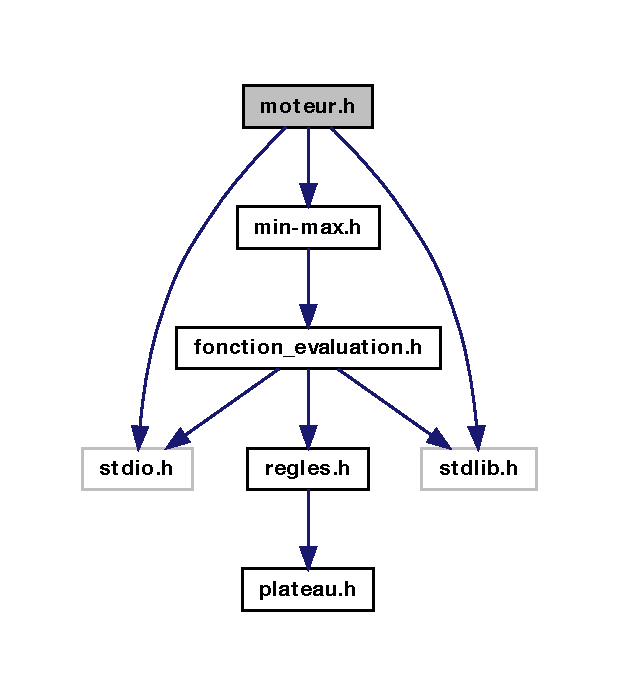
\includegraphics[width=297pt]{moteur_8h__incl}
\end{center}
\end{figure}
Ce graphe montre quels fichiers incluent directement ou indirectement ce fichier :
\nopagebreak
\begin{figure}[H]
\begin{center}
\leavevmode
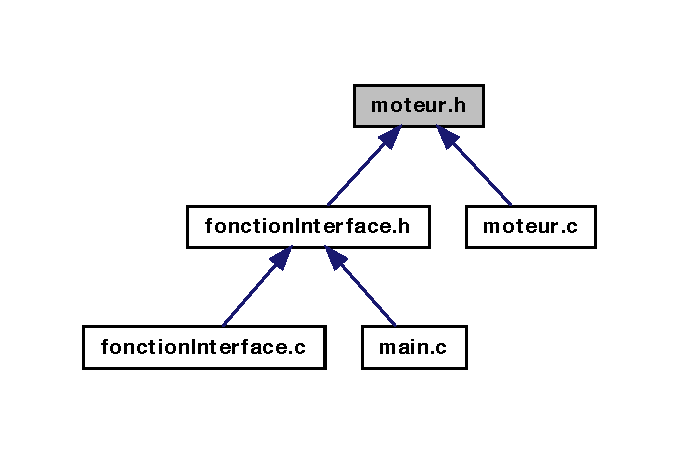
\includegraphics[width=326pt]{moteur_8h__dep__incl}
\end{center}
\end{figure}
\subsection*{Fonctions}
\begin{DoxyCompactItemize}
\item 
void \hyperlink{moteur_8h_a3389f0c85c80a7a201d7f546951c22dd}{initialiser\_\-partie} ()
\begin{DoxyCompactList}\small\item\em Initialise une nouvelle partie, par défaut une partie 2 joueurs, le joueur pourra ensuite être piloté par l'IA en changeant son type grâce à la fonction \hyperlink{moteur_8h_af4cec21f33aec035009dd524c62a13cd}{set\_\-joueur\_\-est\_\-humain}. \item\end{DoxyCompactList}\item 
void \hyperlink{moteur_8h_af4cec21f33aec035009dd524c62a13cd}{set\_\-joueur\_\-est\_\-humain} (\hyperlink{plateau_8h_a8282be6127518547fa916dd6cfef17cb}{couleur\_\-pion} couleur, int boolean)
\begin{DoxyCompactList}\small\item\em Change le type humain ou IA du joueur. \item\end{DoxyCompactList}\item 
\hyperlink{structplateau}{plateau} \hyperlink{moteur_8h_a58e7aeb8e134591ec3402655832840da}{get\_\-plateau} ()
\begin{DoxyCompactList}\small\item\em Renvoie le plateau de la partie pour le consulter. \item\end{DoxyCompactList}\item 
int \hyperlink{moteur_8h_a9ae4819df5eb9b6f1de826520bf30a8b}{sauvegarder\_\-partie} (char $\ast$filename)
\begin{DoxyCompactList}\small\item\em Sauvegarde l'état courant de la partie. \item\end{DoxyCompactList}\item 
int \hyperlink{moteur_8h_a614f6676a1441e96574b1b3f9f5aa7e3}{charger\_\-partie} (char $\ast$filename)
\begin{DoxyCompactList}\small\item\em Charge une partie depuis le disque. \item\end{DoxyCompactList}\item 
int \hyperlink{moteur_8h_afd3360329886ee6f8e2a71a172a4a808}{jouer\_\-coup} (int depart, int arrivee)
\begin{DoxyCompactList}\small\item\em Joue le coup pour le joueur courant. \item\end{DoxyCompactList}\item 
\hypertarget{moteur_8h_af7d1220f033250ed0a11d3669c04d1eb}{
int {\bfseries jouer\_\-coup\_\-xy} (int x1, int y1, int x2, int y2)}
\label{moteur_8h_af7d1220f033250ed0a11d3669c04d1eb}

\item 
void \hyperlink{moteur_8h_acbf0cd12ea068c0f938e62f72419cdcc}{jouer\_\-tour\_\-ia} ()
\begin{DoxyCompactList}\small\item\em Fait jouer un tour à l'IA. \item\end{DoxyCompactList}\item 
void \hyperlink{moteur_8h_a79cf9ff033c4ceaaf0834ad3e51dc37f}{set\_\-difficulte} (int i)
\begin{DoxyCompactList}\small\item\em Joue sur la profondeur d'évaluation du min-\/max. \item\end{DoxyCompactList}\item 
int \hyperlink{moteur_8h_a93014f8aa2a4cb59bdcf0ba5054e86f5}{commencer\_\-tour} ()
\begin{DoxyCompactList}\small\item\em Débute un nouveau tour de jeu, fait jouer l'IA si c'est à elle de jouer, attend un coup humain sinon. \item\end{DoxyCompactList}\item 
void \hyperlink{moteur_8h_a269e871cb87e7db65e8b7a22914275d0}{hint\_\-pions\_\-jouables} ()
\begin{DoxyCompactList}\small\item\em Met en surbrillance les pions qui permettent un déplacement valide pour ce tour. \item\end{DoxyCompactList}\item 
int \hyperlink{moteur_8h_ae85868ec466abc3d96eca06998a01a7d}{hint\_\-deplacements\_\-possibles} (int c)
\begin{DoxyCompactList}\small\item\em Met en surbrillance les déplacements possibles partant d'une case donnée. \item\end{DoxyCompactList}\item 
\hypertarget{moteur_8h_ab7a8dc3359ab20fc1f00616ebd4b47a5}{
int \hyperlink{moteur_8h_ab7a8dc3359ab20fc1f00616ebd4b47a5}{hint\_\-deplacements\_\-possibles\_\-xy} (int x, int y)}
\label{moteur_8h_ab7a8dc3359ab20fc1f00616ebd4b47a5}

\begin{DoxyCompactList}\small\item\em Identique à \hyperlink{moteur_8h_ae85868ec466abc3d96eca06998a01a7d}{hint\_\-deplacements\_\-possibles(int c)} mais prends les coordonnées (x,y) de la case. \item\end{DoxyCompactList}\item 
void \hyperlink{moteur_8h_a5bd6ce9a1afa1f06549fb5aa8a6c40f0}{hint\_\-meilleur\_\-coup} ()
\begin{DoxyCompactList}\small\item\em Met en surbrillance le meilleur coup à jouer en utilisant l'IA. \item\end{DoxyCompactList}\item 
int \hyperlink{moteur_8h_a2836a0f283794670b04163df9027bbc2}{partie\_\-terminee} ()
\end{DoxyCompactItemize}
\subsection*{Variables}
\begin{DoxyCompactItemize}
\item 
\hyperlink{structplateau}{plateau} \hyperlink{moteur_8h_a3efa8d0f7c65daedc584dc8db048e62c}{p\_\-jeu}
\end{DoxyCompactItemize}


\subsection{Description détaillée}
Le moteur de jeu. Il permet de gérer une partie, 1 ou 2 joueurs, fait jouer l'IA, fournit une aide au joueur. \begin{DoxyAuthor}{Auteur}
Mehdi M'rah 

Bastien Auda 
\end{DoxyAuthor}


Définition dans le fichier \hyperlink{moteur_8h_source}{moteur.h}.



\subsection{Documentation des fonctions}
\hypertarget{moteur_8h_a614f6676a1441e96574b1b3f9f5aa7e3}{
\index{moteur.h@{moteur.h}!charger\_\-partie@{charger\_\-partie}}
\index{charger\_\-partie@{charger\_\-partie}!moteur.h@{moteur.h}}
\subsubsection[{charger\_\-partie}]{\setlength{\rightskip}{0pt plus 5cm}int charger\_\-partie (
\begin{DoxyParamCaption}
\item[{char $\ast$}]{filename}
\end{DoxyParamCaption}
)}}
\label{moteur_8h_a614f6676a1441e96574b1b3f9f5aa7e3}


Charge une partie depuis le disque. 


\begin{DoxyParams}{Paramètres}
{\em filename} & Le chemin vers le fichier à charger. \\
\hline
\end{DoxyParams}
\begin{DoxyReturn}{Renvoie}
Vrai si le chargement s'est bien déroulé, faux sinon. 
\end{DoxyReturn}
\begin{DoxyAuthor}{Auteur}
Mehdi M'rah 
\end{DoxyAuthor}


Définition à la ligne \hyperlink{moteur_8c_source_l00249}{249} du fichier \hyperlink{moteur_8c_source}{moteur.c}.

\hypertarget{moteur_8h_a93014f8aa2a4cb59bdcf0ba5054e86f5}{
\index{moteur.h@{moteur.h}!commencer\_\-tour@{commencer\_\-tour}}
\index{commencer\_\-tour@{commencer\_\-tour}!moteur.h@{moteur.h}}
\subsubsection[{commencer\_\-tour}]{\setlength{\rightskip}{0pt plus 5cm}int commencer\_\-tour (
\begin{DoxyParamCaption}
{}
\end{DoxyParamCaption}
)}}
\label{moteur_8h_a93014f8aa2a4cb59bdcf0ba5054e86f5}


Débute un nouveau tour de jeu, fait jouer l'IA si c'est à elle de jouer, attend un coup humain sinon. 

\begin{DoxyReturn}{Renvoie}
Faux si on attend q'un humain joue, vrai si l'IA à joué et qu'on doit relancer immédiatement un nouveau tour. 
\end{DoxyReturn}
\begin{DoxyAuthor}{Auteur}
Bastien Auda 
\end{DoxyAuthor}


Définition à la ligne \hyperlink{moteur_8c_source_l00107}{107} du fichier \hyperlink{moteur_8c_source}{moteur.c}.

\hypertarget{moteur_8h_a58e7aeb8e134591ec3402655832840da}{
\index{moteur.h@{moteur.h}!get\_\-plateau@{get\_\-plateau}}
\index{get\_\-plateau@{get\_\-plateau}!moteur.h@{moteur.h}}
\subsubsection[{get\_\-plateau}]{\setlength{\rightskip}{0pt plus 5cm}{\bf plateau} get\_\-plateau (
\begin{DoxyParamCaption}
{}
\end{DoxyParamCaption}
)}}
\label{moteur_8h_a58e7aeb8e134591ec3402655832840da}


Renvoie le plateau de la partie pour le consulter. 

\begin{DoxyAuthor}{Auteur}
Mehdi M'rah 
\end{DoxyAuthor}


Définition à la ligne \hyperlink{moteur_8c_source_l00351}{351} du fichier \hyperlink{moteur_8c_source}{moteur.c}.

\hypertarget{moteur_8h_ae85868ec466abc3d96eca06998a01a7d}{
\index{moteur.h@{moteur.h}!hint\_\-deplacements\_\-possibles@{hint\_\-deplacements\_\-possibles}}
\index{hint\_\-deplacements\_\-possibles@{hint\_\-deplacements\_\-possibles}!moteur.h@{moteur.h}}
\subsubsection[{hint\_\-deplacements\_\-possibles}]{\setlength{\rightskip}{0pt plus 5cm}int hint\_\-deplacements\_\-possibles (
\begin{DoxyParamCaption}
\item[{int}]{c}
\end{DoxyParamCaption}
)}}
\label{moteur_8h_ae85868ec466abc3d96eca06998a01a7d}


Met en surbrillance les déplacements possibles partant d'une case donnée. 


\begin{DoxyParams}{Paramètres}
{\em c} & Notation officielle de la case de départ. \\
\hline
\end{DoxyParams}
\begin{DoxyReturn}{Renvoie}
Vrai si le pion séléctionné fait partie d'un coup authorisé. 
\end{DoxyReturn}
\begin{DoxyAuthor}{Auteur}
Bastien Auda 
\end{DoxyAuthor}


Définition à la ligne \hyperlink{moteur_8c_source_l00154}{154} du fichier \hyperlink{moteur_8c_source}{moteur.c}.

\hypertarget{moteur_8h_a5bd6ce9a1afa1f06549fb5aa8a6c40f0}{
\index{moteur.h@{moteur.h}!hint\_\-meilleur\_\-coup@{hint\_\-meilleur\_\-coup}}
\index{hint\_\-meilleur\_\-coup@{hint\_\-meilleur\_\-coup}!moteur.h@{moteur.h}}
\subsubsection[{hint\_\-meilleur\_\-coup}]{\setlength{\rightskip}{0pt plus 5cm}void hint\_\-meilleur\_\-coup (
\begin{DoxyParamCaption}
{}
\end{DoxyParamCaption}
)}}
\label{moteur_8h_a5bd6ce9a1afa1f06549fb5aa8a6c40f0}


Met en surbrillance le meilleur coup à jouer en utilisant l'IA. 

\begin{DoxyAuthor}{Auteur}
Mehdi M'rah 
\end{DoxyAuthor}
\hypertarget{moteur_8h_a269e871cb87e7db65e8b7a22914275d0}{
\index{moteur.h@{moteur.h}!hint\_\-pions\_\-jouables@{hint\_\-pions\_\-jouables}}
\index{hint\_\-pions\_\-jouables@{hint\_\-pions\_\-jouables}!moteur.h@{moteur.h}}
\subsubsection[{hint\_\-pions\_\-jouables}]{\setlength{\rightskip}{0pt plus 5cm}void hint\_\-pions\_\-jouables (
\begin{DoxyParamCaption}
{}
\end{DoxyParamCaption}
)}}
\label{moteur_8h_a269e871cb87e7db65e8b7a22914275d0}


Met en surbrillance les pions qui permettent un déplacement valide pour ce tour. 

\begin{DoxyAuthor}{Auteur}
Bastien Auda 
\end{DoxyAuthor}


Définition à la ligne \hyperlink{moteur_8c_source_l00142}{142} du fichier \hyperlink{moteur_8c_source}{moteur.c}.

\hypertarget{moteur_8h_a3389f0c85c80a7a201d7f546951c22dd}{
\index{moteur.h@{moteur.h}!initialiser\_\-partie@{initialiser\_\-partie}}
\index{initialiser\_\-partie@{initialiser\_\-partie}!moteur.h@{moteur.h}}
\subsubsection[{initialiser\_\-partie}]{\setlength{\rightskip}{0pt plus 5cm}void initialiser\_\-partie (
\begin{DoxyParamCaption}
{}
\end{DoxyParamCaption}
)}}
\label{moteur_8h_a3389f0c85c80a7a201d7f546951c22dd}


Initialise une nouvelle partie, par défaut une partie 2 joueurs, le joueur pourra ensuite être piloté par l'IA en changeant son type grâce à la fonction \hyperlink{moteur_8h_af4cec21f33aec035009dd524c62a13cd}{set\_\-joueur\_\-est\_\-humain}. 

void \hyperlink{moteur_8h_a3389f0c85c80a7a201d7f546951c22dd}{initialiser\_\-partie()}; \begin{DoxyAuthor}{Auteur}
Mehdi M'rah 
\end{DoxyAuthor}


Définition à la ligne \hyperlink{moteur_8c_source_l00325}{325} du fichier \hyperlink{moteur_8c_source}{moteur.c}.

\hypertarget{moteur_8h_afd3360329886ee6f8e2a71a172a4a808}{
\index{moteur.h@{moteur.h}!jouer\_\-coup@{jouer\_\-coup}}
\index{jouer\_\-coup@{jouer\_\-coup}!moteur.h@{moteur.h}}
\subsubsection[{jouer\_\-coup}]{\setlength{\rightskip}{0pt plus 5cm}int jouer\_\-coup (
\begin{DoxyParamCaption}
\item[{int}]{depart, }
\item[{int}]{arrivee}
\end{DoxyParamCaption}
)}}
\label{moteur_8h_afd3360329886ee6f8e2a71a172a4a808}


Joue le coup pour le joueur courant. 


\begin{DoxyParams}{Paramètres}
{\em depart} & La case de départ du coup. \\
\hline
{\em arrivee} & La case d'arrivée du coup. \\
\hline
\end{DoxyParams}
\begin{DoxyReturn}{Renvoie}
\begin{DoxyItemize}
\item 0 si le coup est invalide. \item 1 si le coup est valide et terminé. \item 2 si le mouvement fait partie d'un coup valide, on attend que le joueur termine son coup par un nouvel appel à cette fonction \hyperlink{moteur_8h_afd3360329886ee6f8e2a71a172a4a808}{jouer\_\-coup}. \end{DoxyItemize}

\end{DoxyReturn}
\begin{DoxyAuthor}{Auteur}
Bastien Auda 
\end{DoxyAuthor}


Définition à la ligne \hyperlink{moteur_8c_source_l00025}{25} du fichier \hyperlink{moteur_8c_source}{moteur.c}.

\hypertarget{moteur_8h_acbf0cd12ea068c0f938e62f72419cdcc}{
\index{moteur.h@{moteur.h}!jouer\_\-tour\_\-ia@{jouer\_\-tour\_\-ia}}
\index{jouer\_\-tour\_\-ia@{jouer\_\-tour\_\-ia}!moteur.h@{moteur.h}}
\subsubsection[{jouer\_\-tour\_\-ia}]{\setlength{\rightskip}{0pt plus 5cm}void jouer\_\-tour\_\-ia (
\begin{DoxyParamCaption}
{}
\end{DoxyParamCaption}
)}}
\label{moteur_8h_acbf0cd12ea068c0f938e62f72419cdcc}


Fait jouer un tour à l'IA. 

\begin{DoxyAuthor}{Auteur}
Bastien Auda 
\end{DoxyAuthor}


Définition à la ligne \hyperlink{moteur_8c_source_l00126}{126} du fichier \hyperlink{moteur_8c_source}{moteur.c}.

\hypertarget{moteur_8h_a2836a0f283794670b04163df9027bbc2}{
\index{moteur.h@{moteur.h}!partie\_\-terminee@{partie\_\-terminee}}
\index{partie\_\-terminee@{partie\_\-terminee}!moteur.h@{moteur.h}}
\subsubsection[{partie\_\-terminee}]{\setlength{\rightskip}{0pt plus 5cm}int partie\_\-terminee (
\begin{DoxyParamCaption}
{}
\end{DoxyParamCaption}
)}}
\label{moteur_8h_a2836a0f283794670b04163df9027bbc2}
\begin{DoxyReturn}{Renvoie}
Renvoie Faux si la partie n'est pas terminée, la couleur gagnante + 1 sinon. 
\end{DoxyReturn}


Définition à la ligne \hyperlink{moteur_8c_source_l00355}{355} du fichier \hyperlink{moteur_8c_source}{moteur.c}.

\hypertarget{moteur_8h_a9ae4819df5eb9b6f1de826520bf30a8b}{
\index{moteur.h@{moteur.h}!sauvegarder\_\-partie@{sauvegarder\_\-partie}}
\index{sauvegarder\_\-partie@{sauvegarder\_\-partie}!moteur.h@{moteur.h}}
\subsubsection[{sauvegarder\_\-partie}]{\setlength{\rightskip}{0pt plus 5cm}int sauvegarder\_\-partie (
\begin{DoxyParamCaption}
\item[{char $\ast$}]{filename}
\end{DoxyParamCaption}
)}}
\label{moteur_8h_a9ae4819df5eb9b6f1de826520bf30a8b}


Sauvegarde l'état courant de la partie. 


\begin{DoxyParams}{Paramètres}
{\em filename} & Le chemin vers le fichier de sauvegarde. \\
\hline
\end{DoxyParams}
\begin{DoxyReturn}{Renvoie}
Vrai si la sauvegarde s'est bien effectuée, faux si un problème est survenu. 
\end{DoxyReturn}
\begin{DoxyAuthor}{Auteur}
Mehdi M'rah 
\end{DoxyAuthor}


Définition à la ligne \hyperlink{moteur_8c_source_l00185}{185} du fichier \hyperlink{moteur_8c_source}{moteur.c}.

\hypertarget{moteur_8h_a79cf9ff033c4ceaaf0834ad3e51dc37f}{
\index{moteur.h@{moteur.h}!set\_\-difficulte@{set\_\-difficulte}}
\index{set\_\-difficulte@{set\_\-difficulte}!moteur.h@{moteur.h}}
\subsubsection[{set\_\-difficulte}]{\setlength{\rightskip}{0pt plus 5cm}void set\_\-difficulte (
\begin{DoxyParamCaption}
\item[{int}]{i}
\end{DoxyParamCaption}
)}}
\label{moteur_8h_a79cf9ff033c4ceaaf0834ad3e51dc37f}


Joue sur la profondeur d'évaluation du min-\/max. 


\begin{DoxyParams}{Paramètres}
{\em i} & La profondeur d'évaluation. \\
\hline
\end{DoxyParams}
\begin{DoxyAuthor}{Auteur}
Bastien Auda 
\end{DoxyAuthor}


Définition à la ligne \hyperlink{moteur_8c_source_l00138}{138} du fichier \hyperlink{moteur_8c_source}{moteur.c}.

\hypertarget{moteur_8h_af4cec21f33aec035009dd524c62a13cd}{
\index{moteur.h@{moteur.h}!set\_\-joueur\_\-est\_\-humain@{set\_\-joueur\_\-est\_\-humain}}
\index{set\_\-joueur\_\-est\_\-humain@{set\_\-joueur\_\-est\_\-humain}!moteur.h@{moteur.h}}
\subsubsection[{set\_\-joueur\_\-est\_\-humain}]{\setlength{\rightskip}{0pt plus 5cm}void set\_\-joueur\_\-est\_\-humain (
\begin{DoxyParamCaption}
\item[{{\bf couleur\_\-pion}}]{couleur, }
\item[{int}]{boolean}
\end{DoxyParamCaption}
)}}
\label{moteur_8h_af4cec21f33aec035009dd524c62a13cd}


Change le type humain ou IA du joueur. 


\begin{DoxyParams}{Paramètres}
{\em couleur} & La couleur du joueur pour lequel on doit changer le type. \\
\hline
{\em boolean} & Vrai si le joueur est humain, faux sinon. \\
\hline
\end{DoxyParams}
\begin{DoxyAuthor}{Auteur}
Mehdi M'rah 
\end{DoxyAuthor}


Définition à la ligne \hyperlink{moteur_8c_source_l00335}{335} du fichier \hyperlink{moteur_8c_source}{moteur.c}.



\subsection{Documentation des variables}
\hypertarget{moteur_8h_a3efa8d0f7c65daedc584dc8db048e62c}{
\index{moteur.h@{moteur.h}!p\_\-jeu@{p\_\-jeu}}
\index{p\_\-jeu@{p\_\-jeu}!moteur.h@{moteur.h}}
\subsubsection[{p\_\-jeu}]{\setlength{\rightskip}{0pt plus 5cm}{\bf plateau} {\bf p\_\-jeu}}}
\label{moteur_8h_a3efa8d0f7c65daedc584dc8db048e62c}
Le plateau de jeu qui sera utilisé tout au long de la partie. (Ne pas utiliser en dehors de \hyperlink{moteur_8c_source}{moteur.c}, utilisez \hyperlink{moteur_8h_a58e7aeb8e134591ec3402655832840da}{get\_\-plateau()}) 

Définition à la ligne \hyperlink{moteur_8h_source_l00013}{13} du fichier \hyperlink{moteur_8h_source}{moteur.h}.


\hypertarget{moteur_8h_source}{
\section{moteur.h}
}

\begin{DoxyCode}
00001 
00008 \textcolor{preprocessor}{#include <stdio.h>}
00009 \textcolor{preprocessor}{#include <stdlib.h>}
00010 \textcolor{preprocessor}{#include "\hyperlink{min-max_8h}{min-max.h}"}
00011 
\hypertarget{moteur_8h_source_l00013}{}\hyperlink{moteur_8h_a3efa8d0f7c65daedc584dc8db048e62c}{00013} \hyperlink{structplateau}{plateau} \hyperlink{moteur_8h_a3efa8d0f7c65daedc584dc8db048e62c}{p_jeu};
00014 
00020 \textcolor{keywordtype}{void} initialiser\_partie();
00021 
00029 \textcolor{keywordtype}{void} set\_joueur\_est\_humain(\hyperlink{plateau_8h_a8282be6127518547fa916dd6cfef17cb}{couleur_pion} couleur, \textcolor{keywordtype}{int} \textcolor{keywordtype}{boolean});
00030 
00031 
00037 \hyperlink{structplateau}{plateau} get\_plateau();
00038 
00046 \textcolor{keywordtype}{int} sauvegarder\_partie(\textcolor{keywordtype}{char} * filename);
00047 
00055 \textcolor{keywordtype}{int} charger\_partie(\textcolor{keywordtype}{char} * filename);
00056 
00067 \textcolor{keywordtype}{int} jouer\_coup(\textcolor{keywordtype}{int} depart, \textcolor{keywordtype}{int} arrivee);
00068 
00073 \textcolor{keywordtype}{int} jouer\_coup\_xy(\textcolor{keywordtype}{int} x1, \textcolor{keywordtype}{int} y1, \textcolor{keywordtype}{int} x2, \textcolor{keywordtype}{int} y2);
00074 
00080 \textcolor{keywordtype}{void} jouer\_tour\_ia();
00081 
00088 \textcolor{keywordtype}{void} set\_difficulte(\textcolor{keywordtype}{int} i);
00089 
00096 \textcolor{keywordtype}{int} commencer\_tour();
00097 
00103 \textcolor{keywordtype}{void} hint\_pions\_jouables();
00104 
00112 \textcolor{keywordtype}{int} hint\_deplacements\_possibles(\textcolor{keywordtype}{int} c);
00113 
00118 \textcolor{keywordtype}{int} hint\_deplacements\_possibles\_xy(\textcolor{keywordtype}{int} \hyperlink{plateau_8h_a9e00f85b4b6ec2d8bdfbe94ff40f0eeeacab1e15e82c5976bfb476ddfe145263c}{x},\textcolor{keywordtype}{int} y);
00119 
00125 \textcolor{keywordtype}{void} \hyperlink{moteur_8h_a5bd6ce9a1afa1f06549fb5aa8a6c40f0}{hint_meilleur_coup}();
00126 
00131 \textcolor{keywordtype}{int} partie\_terminee();
\end{DoxyCode}

\hypertarget{plateau_8h}{
\section{Référence du fichier plateau.h}
\label{plateau_8h}\index{plateau.h@{plateau.h}}
}


Tout ce qui concerne le plateau de jeu (damier, pions et joueurs).  


Ce graphe montre quels fichiers incluent directement ou indirectement ce fichier :
\nopagebreak
\begin{figure}[H]
\begin{center}
\leavevmode
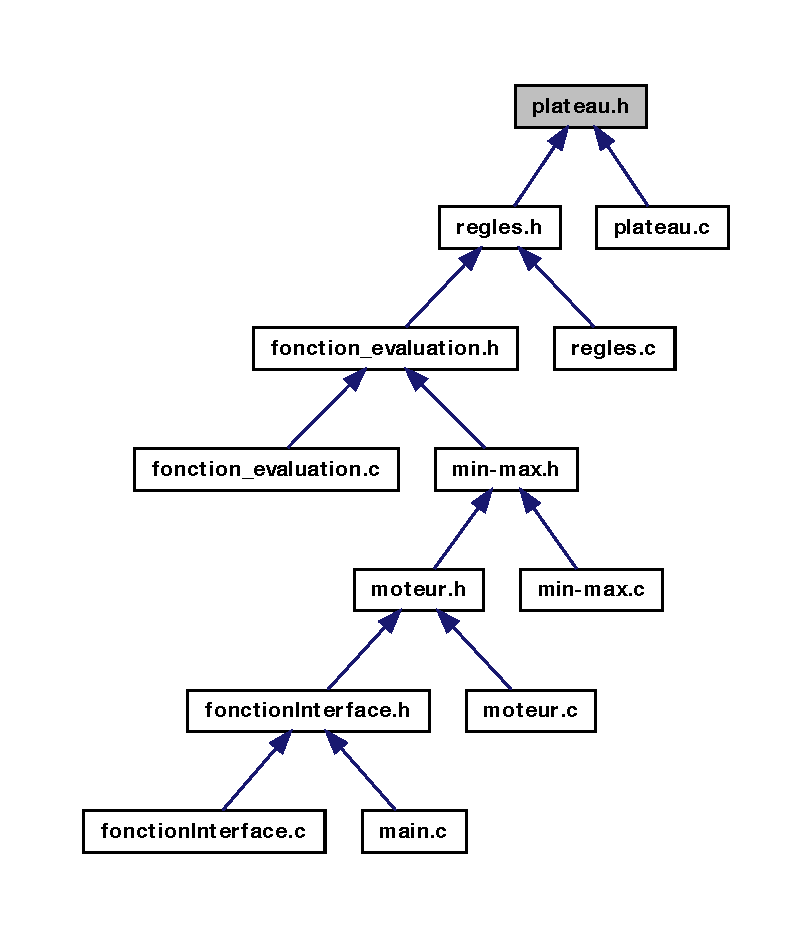
\includegraphics[width=389pt]{plateau_8h__dep__incl}
\end{center}
\end{figure}
\subsection*{Structures de données}
\begin{DoxyCompactItemize}
\item 
struct \hyperlink{structpion}{pion}
\begin{DoxyCompactList}\small\item\em Objet pion. Un pion est déterminé par une couleur et si il est une dame ou non. \item\end{DoxyCompactList}\item 
struct \hyperlink{structcase__plateau}{case\_\-plateau}
\begin{DoxyCompactList}\small\item\em Objet case du plateau de jeu. Une case est définie par une couleur et, si elle est noire,elle dispose d'une abscisse (x) et une ordonnée (y) sur le plateau. Une case peut être libre ou non, si elle n'est pas libre elle contient un pion. \item\end{DoxyCompactList}\item 
struct \hyperlink{structjoueur}{joueur}
\begin{DoxyCompactList}\small\item\em Objet joueur. Un joueur est caractérisé par la couleur qu'il joue et sa nature (humain ou intelligence artificielle). \item\end{DoxyCompactList}\item 
struct \hyperlink{structcoup}{coup}
\begin{DoxyCompactList}\small\item\em Objet coup. Un coup est défini par un numéro de case de départ, un numéro de case d'arrivée, un type (déplacement ou prise) et optinellement un commentaire. \item\end{DoxyCompactList}\item 
struct \hyperlink{structplateau}{plateau}
\begin{DoxyCompactList}\small\item\em Objet plateau. Le plateau est composé de 50 cases, numérotées de 1 à 50. Il comporte un historique des coups. Il sait quel joueur doit jouer le prochain coup. \item\end{DoxyCompactList}\end{DoxyCompactItemize}
\subsection*{Énumérations}
\begin{DoxyCompactItemize}
\item 
enum \hyperlink{plateau_8h_a8282be6127518547fa916dd6cfef17cb}{couleur\_\-pion} \{ {\bfseries blanc}, 
{\bfseries noir}
 \}
\begin{DoxyCompactList}\small\item\em La couleur d'un pion. \item\end{DoxyCompactList}\item 
enum \hyperlink{plateau_8h_a9e00f85b4b6ec2d8bdfbe94ff40f0eee}{type\_\-coup} \{ \hyperlink{plateau_8h_a9e00f85b4b6ec2d8bdfbe94ff40f0eeeacab1e15e82c5976bfb476ddfe145263c}{x}, 
\hyperlink{plateau_8h_a9e00f85b4b6ec2d8bdfbe94ff40f0eeea0247320c476fffeaa81ffa7836e08dee}{t}
 \}
\begin{DoxyCompactList}\small\item\em Le type de coup. Le \char`\"{}tiret\char`\"{} '-\/' est remplacé par un 't'. \item\end{DoxyCompactList}\end{DoxyCompactItemize}
\subsection*{Fonctions}
\begin{DoxyCompactItemize}
\item 
\hyperlink{structplateau}{plateau} \hyperlink{plateau_8h_aad79656ee484352eb698011738cbcefc}{nouveau\_\-plateau} (\hyperlink{structjoueur}{joueur} j1, \hyperlink{structjoueur}{joueur} j2)
\begin{DoxyCompactList}\small\item\em Fonction de création d'un nouveau plateau. \item\end{DoxyCompactList}\item 
int \hyperlink{plateau_8h_ac36612024e6663243c4f0605f2dd96c2}{plateau\_\-deplacer\_\-pion} (int old\_\-position, int new\_\-position, \hyperlink{structplateau}{plateau} $\ast$p)
\begin{DoxyCompactList}\small\item\em Déplace un pion. \item\end{DoxyCompactList}\item 
int \hyperlink{plateau_8h_a4a8fb7c96fbeb8218d5ddbf3fe642901}{plateau\_\-prendre\_\-pion} (int position, \hyperlink{structplateau}{plateau} $\ast$p)
\begin{DoxyCompactList}\small\item\em Prend le pion de la case \char`\"{}position\char`\"{}. \item\end{DoxyCompactList}\item 
void \hyperlink{plateau_8h_a8e9db1b793881c55d1261e3b735a5d48}{plateau\_\-ajouter\_\-coup} (\hyperlink{structcoup}{coup} c, \hyperlink{structplateau}{plateau} $\ast$p)
\begin{DoxyCompactList}\small\item\em Ajoute un coup dans l'historique du plateau. \item\end{DoxyCompactList}\item 
void \hyperlink{plateau_8h_a6616eb0e3e305b9dd718ffb0e83231d5}{plateau\_\-appliquer\_\-coup} (\hyperlink{structcoup}{coup} c, \hyperlink{structplateau}{plateau} $\ast$p)
\begin{DoxyCompactList}\small\item\em Met à jour le plateau en jouant le coup donné et passe la main au joueur suivant. \item\end{DoxyCompactList}\item 
int \hyperlink{plateau_8h_a43fa8dd4c36ca967403900b75237a3d5}{plateau\_\-partie\_\-finie} (\hyperlink{structplateau}{plateau} p)
\begin{DoxyCompactList}\small\item\em Teste si la partie est gagnée pour un des deux joueurs. \item\end{DoxyCompactList}\item 
\hyperlink{structcase__plateau}{case\_\-plateau} \hyperlink{plateau_8h_a44f4edc5041fe92213f7dbdc2ac5e39e}{get\_\-case\_\-plateau} (int x, int y, \hyperlink{structplateau}{plateau} p)
\begin{DoxyCompactList}\small\item\em Renvoie la case à la position (x,y). \item\end{DoxyCompactList}\item 
void \hyperlink{plateau_8h_a69dc99f7c855cdf8bf569f8b26ae6689}{print\_\-case} (\hyperlink{structcase__plateau}{case\_\-plateau} c)
\begin{DoxyCompactList}\small\item\em Affiche les informations sur la case (à des fins de test). \item\end{DoxyCompactList}\item 
\hypertarget{plateau_8h_a590ca6fc3ab1b4e08fa05ddaf7465115}{
void \hyperlink{plateau_8h_a590ca6fc3ab1b4e08fa05ddaf7465115}{print\_\-plateau} (\hyperlink{structplateau}{plateau} p)}
\label{plateau_8h_a590ca6fc3ab1b4e08fa05ddaf7465115}

\begin{DoxyCompactList}\small\item\em Affiche le plateau sur stdout. \item\end{DoxyCompactList}\item 
void \hyperlink{plateau_8h_a4066fdb86d7d54a9256fa727995f47fd}{set\_\-case\_\-en\_\-surbrillance} (int numero, \hyperlink{structplateau}{plateau} $\ast$p)
\begin{DoxyCompactList}\small\item\em Met la case en surbrillance. \item\end{DoxyCompactList}\item 
void \hyperlink{plateau_8h_a98033598d0f16369d8529f7c5ab3e3fd}{set\_\-pion\_\-en\_\-surbrillance} (int numero, \hyperlink{structplateau}{plateau} $\ast$p)
\begin{DoxyCompactList}\small\item\em Met un pion en surbrillance. \item\end{DoxyCompactList}\item 
\hypertarget{plateau_8h_aee51bfad885420a7013c9c01a2eae048}{
void \hyperlink{plateau_8h_aee51bfad885420a7013c9c01a2eae048}{reset\_\-surbrillance} (\hyperlink{structplateau}{plateau} $\ast$p)}
\label{plateau_8h_aee51bfad885420a7013c9c01a2eae048}

\begin{DoxyCompactList}\small\item\em Annule la mise en surbrillance de toutes les cases et tous les pions du plateau. \item\end{DoxyCompactList}\item 
void \hyperlink{plateau_8h_a5b1f6227bf2bab71a07a531c49270b51}{printCoup} (const \hyperlink{structcoup}{coup} c)
\begin{DoxyCompactList}\small\item\em print les infos d'un coup \item\end{DoxyCompactList}\item 
int \hyperlink{plateau_8h_aff9fd9b1b3f96bbae116f3d87349a0cf}{est\_\-prenable} (int position, \hyperlink{structplateau}{plateau} $\ast$p)
\begin{DoxyCompactList}\small\item\em predicat pour savoir si une position est prenable. \item\end{DoxyCompactList}\item 
void \hyperlink{plateau_8h_ade9b690d9493e82b264dcea4d08abd5a}{print\_\-liste\_\-coups} (\hyperlink{structcoup}{coup} $\ast$l)
\begin{DoxyCompactList}\small\item\em affiche la liste des coups dans l. \item\end{DoxyCompactList}\item 
\hypertarget{plateau_8h_a66fb3aa869ea21274bd48d004fbd6110}{
int {\bfseries coup\_\-inclus} (\hyperlink{structcase__plateau}{case\_\-plateau} c, \hyperlink{structcase__plateau}{case\_\-plateau} $\ast$liste, int taille)}
\label{plateau_8h_a66fb3aa869ea21274bd48d004fbd6110}

\item 
\hyperlink{structcase__plateau}{case\_\-plateau} \hyperlink{plateau_8h_a60a8f706865d0ae9087f8d65d4667655}{get\_\-case\_\-plateau\_\-silent} (int x, int y, \hyperlink{structplateau}{plateau} p)
\begin{DoxyCompactList}\small\item\em retourne la case si elle existe, ou la case 0 sinon \item\end{DoxyCompactList}\item 
int \hyperlink{plateau_8h_a8918a9186794792439622dd39ca202a0}{nombre\_\-coups} (\hyperlink{structcoup}{coup} $\ast$set)
\begin{DoxyCompactList}\small\item\em retourne le nombre de coups dans set \item\end{DoxyCompactList}\end{DoxyCompactItemize}


\subsection{Description détaillée}
Tout ce qui concerne le plateau de jeu (damier, pions et joueurs). \begin{DoxyAuthor}{Auteur}
Bastien Auda 
\end{DoxyAuthor}


Définition dans le fichier \hyperlink{plateau_8h_source}{plateau.h}.



\subsection{Documentation du type de l'énumération}
\hypertarget{plateau_8h_a9e00f85b4b6ec2d8bdfbe94ff40f0eee}{
\index{plateau.h@{plateau.h}!type\_\-coup@{type\_\-coup}}
\index{type\_\-coup@{type\_\-coup}!plateau.h@{plateau.h}}
\subsubsection[{type\_\-coup}]{\setlength{\rightskip}{0pt plus 5cm}enum {\bf type\_\-coup}}}
\label{plateau_8h_a9e00f85b4b6ec2d8bdfbe94ff40f0eee}


Le type de coup. Le \char`\"{}tiret\char`\"{} '-\/' est remplacé par un 't'. 

\begin{Desc}
\item[Valeurs énumérées: ]\par
\begin{description}
\index{x@{x}!plateau.h@{plateau.h}}\index{plateau.h@{plateau.h}!x@{x}}\item[{\em 
\hypertarget{plateau_8h_a9e00f85b4b6ec2d8bdfbe94ff40f0eeeacab1e15e82c5976bfb476ddfe145263c}{
x}
\label{plateau_8h_a9e00f85b4b6ec2d8bdfbe94ff40f0eeeacab1e15e82c5976bfb476ddfe145263c}
}]Prise. \index{t@{t}!plateau.h@{plateau.h}}\index{plateau.h@{plateau.h}!t@{t}}\item[{\em 
\hypertarget{plateau_8h_a9e00f85b4b6ec2d8bdfbe94ff40f0eeea0247320c476fffeaa81ffa7836e08dee}{
t}
\label{plateau_8h_a9e00f85b4b6ec2d8bdfbe94ff40f0eeea0247320c476fffeaa81ffa7836e08dee}
}]Déplacement. \end{description}
\end{Desc}



Définition à la ligne \hyperlink{plateau_8h_source_l00022}{22} du fichier \hyperlink{plateau_8h_source}{plateau.h}.



\subsection{Documentation des fonctions}
\hypertarget{plateau_8h_aff9fd9b1b3f96bbae116f3d87349a0cf}{
\index{plateau.h@{plateau.h}!est\_\-prenable@{est\_\-prenable}}
\index{est\_\-prenable@{est\_\-prenable}!plateau.h@{plateau.h}}
\subsubsection[{est\_\-prenable}]{\setlength{\rightskip}{0pt plus 5cm}int est\_\-prenable (
\begin{DoxyParamCaption}
\item[{int}]{position, }
\item[{{\bf plateau} $\ast$}]{p}
\end{DoxyParamCaption}
)}}
\label{plateau_8h_aff9fd9b1b3f96bbae116f3d87349a0cf}


predicat pour savoir si une position est prenable. 


\begin{DoxyParams}{Paramètres}
{\em position} & la position du pion que l'on veut prendre. \\
\hline
{\em p} & le plateau sur lequel on veut tester la position à prendre. \\
\hline
\end{DoxyParams}


Définition à la ligne \hyperlink{plateau_8c_source_l00258}{258} du fichier \hyperlink{plateau_8c_source}{plateau.c}.

\hypertarget{plateau_8h_a44f4edc5041fe92213f7dbdc2ac5e39e}{
\index{plateau.h@{plateau.h}!get\_\-case\_\-plateau@{get\_\-case\_\-plateau}}
\index{get\_\-case\_\-plateau@{get\_\-case\_\-plateau}!plateau.h@{plateau.h}}
\subsubsection[{get\_\-case\_\-plateau}]{\setlength{\rightskip}{0pt plus 5cm}{\bf case\_\-plateau} get\_\-case\_\-plateau (
\begin{DoxyParamCaption}
\item[{int}]{x, }
\item[{int}]{y, }
\item[{{\bf plateau}}]{p}
\end{DoxyParamCaption}
)}}
\label{plateau_8h_a44f4edc5041fe92213f7dbdc2ac5e39e}


Renvoie la case à la position (x,y). 


\begin{DoxyParams}{Paramètres}
{\em x} & Abscisse de la case (colonne) \mbox{[}1-\/10\mbox{]}. \\
\hline
{\em y} & Ordonnée de la case \mbox{[}1-\/10\mbox{]}. \\
\hline
\end{DoxyParams}


Définition à la ligne \hyperlink{plateau_8c_source_l00101}{101} du fichier \hyperlink{plateau_8c_source}{plateau.c}.

\hypertarget{plateau_8h_a60a8f706865d0ae9087f8d65d4667655}{
\index{plateau.h@{plateau.h}!get\_\-case\_\-plateau\_\-silent@{get\_\-case\_\-plateau\_\-silent}}
\index{get\_\-case\_\-plateau\_\-silent@{get\_\-case\_\-plateau\_\-silent}!plateau.h@{plateau.h}}
\subsubsection[{get\_\-case\_\-plateau\_\-silent}]{\setlength{\rightskip}{0pt plus 5cm}{\bf case\_\-plateau} get\_\-case\_\-plateau\_\-silent (
\begin{DoxyParamCaption}
\item[{int}]{x, }
\item[{int}]{y, }
\item[{{\bf plateau}}]{p}
\end{DoxyParamCaption}
)}}
\label{plateau_8h_a60a8f706865d0ae9087f8d65d4667655}


retourne la case si elle existe, ou la case 0 sinon 


\begin{DoxyParams}{Paramètres}
{\em x} & la position horizontale sur le plateau \\
\hline
{\em y} & la position verticale sur le plateau \\
\hline
{\em p} & le plateau courant \\
\hline
\end{DoxyParams}
\begin{DoxyAuthor}{Auteur}
Paraita Wohler
\end{DoxyAuthor}

\begin{DoxyParams}{Paramètres}
{\em x} & la position en abscisse \\
\hline
{\em y} & la position en ordonnée \\
\hline
{\em p} & le plateau courant \\
\hline
\end{DoxyParams}
\begin{DoxyReturn}{Renvoie}
la case qui est en position x y dans p 
\end{DoxyReturn}


Définition à la ligne \hyperlink{regles_8c_source_l00929}{929} du fichier \hyperlink{regles_8c_source}{regles.c}.

\hypertarget{plateau_8h_a8918a9186794792439622dd39ca202a0}{
\index{plateau.h@{plateau.h}!nombre\_\-coups@{nombre\_\-coups}}
\index{nombre\_\-coups@{nombre\_\-coups}!plateau.h@{plateau.h}}
\subsubsection[{nombre\_\-coups}]{\setlength{\rightskip}{0pt plus 5cm}int nombre\_\-coups (
\begin{DoxyParamCaption}
\item[{{\bf coup} $\ast$}]{set}
\end{DoxyParamCaption}
)}}
\label{plateau_8h_a8918a9186794792439622dd39ca202a0}


retourne le nombre de coups dans set 


\begin{DoxyParams}{Paramètres}
{\em set} & le tableau des coups. \\
\hline
\end{DoxyParams}
\begin{DoxyAuthor}{Auteur}
Paraita Wohler 
\end{DoxyAuthor}


Définition à la ligne \hyperlink{plateau_8c_source_l00300}{300} du fichier \hyperlink{plateau_8c_source}{plateau.c}.

\hypertarget{plateau_8h_aad79656ee484352eb698011738cbcefc}{
\index{plateau.h@{plateau.h}!nouveau\_\-plateau@{nouveau\_\-plateau}}
\index{nouveau\_\-plateau@{nouveau\_\-plateau}!plateau.h@{plateau.h}}
\subsubsection[{nouveau\_\-plateau}]{\setlength{\rightskip}{0pt plus 5cm}{\bf plateau} nouveau\_\-plateau (
\begin{DoxyParamCaption}
\item[{{\bf joueur}}]{j1, }
\item[{{\bf joueur}}]{j2}
\end{DoxyParamCaption}
)}}
\label{plateau_8h_aad79656ee484352eb698011738cbcefc}


Fonction de création d'un nouveau plateau. 


\begin{DoxyParams}{Paramètres}
{\em j1} & Le joueur blanc. \\
\hline
{\em j2} & Le joueur noir. \\
\hline
\end{DoxyParams}
\begin{DoxyReturn}{Renvoie}
plateau Un plateau initialisé avec les pions en position initiale et associé aux joueurs. 
\end{DoxyReturn}


Définition à la ligne \hyperlink{plateau_8c_source_l00011}{11} du fichier \hyperlink{plateau_8c_source}{plateau.c}.

\hypertarget{plateau_8h_a8e9db1b793881c55d1261e3b735a5d48}{
\index{plateau.h@{plateau.h}!plateau\_\-ajouter\_\-coup@{plateau\_\-ajouter\_\-coup}}
\index{plateau\_\-ajouter\_\-coup@{plateau\_\-ajouter\_\-coup}!plateau.h@{plateau.h}}
\subsubsection[{plateau\_\-ajouter\_\-coup}]{\setlength{\rightskip}{0pt plus 5cm}void plateau\_\-ajouter\_\-coup (
\begin{DoxyParamCaption}
\item[{{\bf coup}}]{c, }
\item[{{\bf plateau} $\ast$}]{p}
\end{DoxyParamCaption}
)}}
\label{plateau_8h_a8e9db1b793881c55d1261e3b735a5d48}


Ajoute un coup dans l'historique du plateau. 


\begin{DoxyParams}{Paramètres}
{\em c} & Le coup à ajouter. \\
\hline
{\em p} & Le plateau auquel on ajoute le coup. En raison du risque improbable qu'une partie dure plus de 500 coups, l'historique au-\/delà est ignoré. \\
\hline
\end{DoxyParams}


Définition à la ligne \hyperlink{plateau_8c_source_l00093}{93} du fichier \hyperlink{plateau_8c_source}{plateau.c}.

\hypertarget{plateau_8h_a6616eb0e3e305b9dd718ffb0e83231d5}{
\index{plateau.h@{plateau.h}!plateau\_\-appliquer\_\-coup@{plateau\_\-appliquer\_\-coup}}
\index{plateau\_\-appliquer\_\-coup@{plateau\_\-appliquer\_\-coup}!plateau.h@{plateau.h}}
\subsubsection[{plateau\_\-appliquer\_\-coup}]{\setlength{\rightskip}{0pt plus 5cm}void plateau\_\-appliquer\_\-coup (
\begin{DoxyParamCaption}
\item[{{\bf coup}}]{c, }
\item[{{\bf plateau} $\ast$}]{p}
\end{DoxyParamCaption}
)}}
\label{plateau_8h_a6616eb0e3e305b9dd718ffb0e83231d5}


Met à jour le plateau en jouant le coup donné et passe la main au joueur suivant. 


\begin{DoxyParams}{Paramètres}
{\em c} & Le coup à jouer. \\
\hline
\end{DoxyParams}


Définition à la ligne \hyperlink{plateau_8c_source_l00141}{141} du fichier \hyperlink{plateau_8c_source}{plateau.c}.

\hypertarget{plateau_8h_ac36612024e6663243c4f0605f2dd96c2}{
\index{plateau.h@{plateau.h}!plateau\_\-deplacer\_\-pion@{plateau\_\-deplacer\_\-pion}}
\index{plateau\_\-deplacer\_\-pion@{plateau\_\-deplacer\_\-pion}!plateau.h@{plateau.h}}
\subsubsection[{plateau\_\-deplacer\_\-pion}]{\setlength{\rightskip}{0pt plus 5cm}int plateau\_\-deplacer\_\-pion (
\begin{DoxyParamCaption}
\item[{int}]{old\_\-position, }
\item[{int}]{new\_\-position, }
\item[{{\bf plateau} $\ast$}]{p}
\end{DoxyParamCaption}
)}}
\label{plateau_8h_ac36612024e6663243c4f0605f2dd96c2}


Déplace un pion. 


\begin{DoxyParams}{Paramètres}
{\em old\_\-position} & La position de départ. \\
\hline
{\em new\_\-position} & La position d'arrivée. \\
\hline
\end{DoxyParams}
\begin{DoxyReturn}{Renvoie}
int Vrai si le déplacement est possible, faux si un pion occupe déjà la case ou si on sort du plateau. 
\end{DoxyReturn}


Définition à la ligne \hyperlink{plateau_8c_source_l00070}{70} du fichier \hyperlink{plateau_8c_source}{plateau.c}.

\hypertarget{plateau_8h_a43fa8dd4c36ca967403900b75237a3d5}{
\index{plateau.h@{plateau.h}!plateau\_\-partie\_\-finie@{plateau\_\-partie\_\-finie}}
\index{plateau\_\-partie\_\-finie@{plateau\_\-partie\_\-finie}!plateau.h@{plateau.h}}
\subsubsection[{plateau\_\-partie\_\-finie}]{\setlength{\rightskip}{0pt plus 5cm}int plateau\_\-partie\_\-finie (
\begin{DoxyParamCaption}
\item[{{\bf plateau}}]{p}
\end{DoxyParamCaption}
)}}
\label{plateau_8h_a43fa8dd4c36ca967403900b75237a3d5}


Teste si la partie est gagnée pour un des deux joueurs. 

\begin{DoxyReturn}{Renvoie}
0 si la partie n'est pas finie, couleur + 1 sinon. 
\end{DoxyReturn}


Définition à la ligne \hyperlink{plateau_8c_source_l00175}{175} du fichier \hyperlink{plateau_8c_source}{plateau.c}.

\hypertarget{plateau_8h_a4a8fb7c96fbeb8218d5ddbf3fe642901}{
\index{plateau.h@{plateau.h}!plateau\_\-prendre\_\-pion@{plateau\_\-prendre\_\-pion}}
\index{plateau\_\-prendre\_\-pion@{plateau\_\-prendre\_\-pion}!plateau.h@{plateau.h}}
\subsubsection[{plateau\_\-prendre\_\-pion}]{\setlength{\rightskip}{0pt plus 5cm}int plateau\_\-prendre\_\-pion (
\begin{DoxyParamCaption}
\item[{int}]{position, }
\item[{{\bf plateau} $\ast$}]{p}
\end{DoxyParamCaption}
)}}
\label{plateau_8h_a4a8fb7c96fbeb8218d5ddbf3fe642901}


Prend le pion de la case \char`\"{}position\char`\"{}. 


\begin{DoxyParams}{Paramètres}
{\em position} & Position de la case sur laquelle se trouve le pion. \\
\hline
\end{DoxyParams}
\begin{DoxyReturn}{Renvoie}
int Vrai si la prise est effectuée, faux si la case est vide ou si on sort du plateau. 
\end{DoxyReturn}


Définition à la ligne \hyperlink{plateau_8c_source_l00084}{84} du fichier \hyperlink{plateau_8c_source}{plateau.c}.

\hypertarget{plateau_8h_a69dc99f7c855cdf8bf569f8b26ae6689}{
\index{plateau.h@{plateau.h}!print\_\-case@{print\_\-case}}
\index{print\_\-case@{print\_\-case}!plateau.h@{plateau.h}}
\subsubsection[{print\_\-case}]{\setlength{\rightskip}{0pt plus 5cm}void print\_\-case (
\begin{DoxyParamCaption}
\item[{{\bf case\_\-plateau}}]{c}
\end{DoxyParamCaption}
)}}
\label{plateau_8h_a69dc99f7c855cdf8bf569f8b26ae6689}


Affiche les informations sur la case (à des fins de test). 


\begin{DoxyParams}{Paramètres}
{\em c} & La case à afficher. \\
\hline
\end{DoxyParams}


Définition à la ligne \hyperlink{plateau_8c_source_l00120}{120} du fichier \hyperlink{plateau_8c_source}{plateau.c}.

\hypertarget{plateau_8h_ade9b690d9493e82b264dcea4d08abd5a}{
\index{plateau.h@{plateau.h}!print\_\-liste\_\-coups@{print\_\-liste\_\-coups}}
\index{print\_\-liste\_\-coups@{print\_\-liste\_\-coups}!plateau.h@{plateau.h}}
\subsubsection[{print\_\-liste\_\-coups}]{\setlength{\rightskip}{0pt plus 5cm}void print\_\-liste\_\-coups (
\begin{DoxyParamCaption}
\item[{{\bf coup} $\ast$}]{l}
\end{DoxyParamCaption}
)}}
\label{plateau_8h_ade9b690d9493e82b264dcea4d08abd5a}


affiche la liste des coups dans l. 


\begin{DoxyParams}{Paramètres}
{\em l} & la liste des coups que l'on veut afficher. \\
\hline
\end{DoxyParams}
\begin{DoxyAuthor}{Auteur}
Paraita Wohler 
\end{DoxyAuthor}


Définition à la ligne \hyperlink{plateau_8c_source_l00269}{269} du fichier \hyperlink{plateau_8c_source}{plateau.c}.

\hypertarget{plateau_8h_a5b1f6227bf2bab71a07a531c49270b51}{
\index{plateau.h@{plateau.h}!printCoup@{printCoup}}
\index{printCoup@{printCoup}!plateau.h@{plateau.h}}
\subsubsection[{printCoup}]{\setlength{\rightskip}{0pt plus 5cm}void printCoup (
\begin{DoxyParamCaption}
\item[{const {\bf coup}}]{c}
\end{DoxyParamCaption}
)}}
\label{plateau_8h_a5b1f6227bf2bab71a07a531c49270b51}


print les infos d'un coup 


\begin{DoxyParams}{Paramètres}
{\em c} & le coup dont on veut les informations. \\
\hline
\end{DoxyParams}
\begin{DoxyAuthor}{Auteur}
Paraita Wohler 
\end{DoxyAuthor}


Définition à la ligne \hyperlink{plateau_8c_source_l00234}{234} du fichier \hyperlink{plateau_8c_source}{plateau.c}.

\hypertarget{plateau_8h_a4066fdb86d7d54a9256fa727995f47fd}{
\index{plateau.h@{plateau.h}!set\_\-case\_\-en\_\-surbrillance@{set\_\-case\_\-en\_\-surbrillance}}
\index{set\_\-case\_\-en\_\-surbrillance@{set\_\-case\_\-en\_\-surbrillance}!plateau.h@{plateau.h}}
\subsubsection[{set\_\-case\_\-en\_\-surbrillance}]{\setlength{\rightskip}{0pt plus 5cm}void set\_\-case\_\-en\_\-surbrillance (
\begin{DoxyParamCaption}
\item[{int}]{numero, }
\item[{{\bf plateau} $\ast$}]{p}
\end{DoxyParamCaption}
)}}
\label{plateau_8h_a4066fdb86d7d54a9256fa727995f47fd}


Met la case en surbrillance. 


\begin{DoxyParams}{Paramètres}
{\em numero} & Numéro de la case à mettre en surbrillance (selon la notation officielle). \\
\hline
\end{DoxyParams}


Définition à la ligne \hyperlink{plateau_8c_source_l00125}{125} du fichier \hyperlink{plateau_8c_source}{plateau.c}.

\hypertarget{plateau_8h_a98033598d0f16369d8529f7c5ab3e3fd}{
\index{plateau.h@{plateau.h}!set\_\-pion\_\-en\_\-surbrillance@{set\_\-pion\_\-en\_\-surbrillance}}
\index{set\_\-pion\_\-en\_\-surbrillance@{set\_\-pion\_\-en\_\-surbrillance}!plateau.h@{plateau.h}}
\subsubsection[{set\_\-pion\_\-en\_\-surbrillance}]{\setlength{\rightskip}{0pt plus 5cm}void set\_\-pion\_\-en\_\-surbrillance (
\begin{DoxyParamCaption}
\item[{int}]{numero, }
\item[{{\bf plateau} $\ast$}]{p}
\end{DoxyParamCaption}
)}}
\label{plateau_8h_a98033598d0f16369d8529f7c5ab3e3fd}


Met un pion en surbrillance. 


\begin{DoxyParams}{Paramètres}
{\em numero} & Numéro de la case sur laquelle se trouve le pion à mettre en surbrillance (selon la notation officielle). \\
\hline
\end{DoxyParams}


Définition à la ligne \hyperlink{plateau_8c_source_l00129}{129} du fichier \hyperlink{plateau_8c_source}{plateau.c}.


\hypertarget{plateau_8h_source}{
\section{plateau.h}
}

\begin{DoxyCode}
00001 
\hypertarget{plateau_8h_source_l00012}{}\hyperlink{plateau_8h_a8282be6127518547fa916dd6cfef17cb}{00012} \textcolor{keyword}{typedef} \textcolor{keyword}{enum} \{
00013         blanc,
00014         noir
00015 \} \hyperlink{plateau_8h_a8282be6127518547fa916dd6cfef17cb}{couleur_pion};
00016 
\hypertarget{plateau_8h_source_l00022}{}\hyperlink{plateau_8h_a9e00f85b4b6ec2d8bdfbe94ff40f0eee}{00022} \textcolor{keyword}{typedef} \textcolor{keyword}{enum} \{
\hypertarget{plateau_8h_source_l00023}{}\hyperlink{plateau_8h_a9e00f85b4b6ec2d8bdfbe94ff40f0eeeacab1e15e82c5976bfb476ddfe145263c}{00023}         \hyperlink{plateau_8h_a9e00f85b4b6ec2d8bdfbe94ff40f0eeeacab1e15e82c5976bfb476ddfe145263c}{x}, 
\hypertarget{plateau_8h_source_l00024}{}\hyperlink{plateau_8h_a9e00f85b4b6ec2d8bdfbe94ff40f0eeea0247320c476fffeaa81ffa7836e08dee}{00024}         \hyperlink{plateau_8h_a9e00f85b4b6ec2d8bdfbe94ff40f0eeea0247320c476fffeaa81ffa7836e08dee}{t} 
00025 \} \hyperlink{plateau_8h_a9e00f85b4b6ec2d8bdfbe94ff40f0eee}{type_coup};
00026 
00027 
\hypertarget{plateau_8h_source_l00033}{}\hyperlink{structpion}{00033} \textcolor{keyword}{typedef} \textcolor{keyword}{struct }\{
00034         \hyperlink{plateau_8h_a8282be6127518547fa916dd6cfef17cb}{couleur_pion} couleur;
\hypertarget{plateau_8h_source_l00035}{}\hyperlink{structpion_a13d497ed763d6eba18df86caf4c85861}{00035}         \textcolor{keywordtype}{int} \hyperlink{structpion_a13d497ed763d6eba18df86caf4c85861}{est_dame};           
\hypertarget{plateau_8h_source_l00036}{}\hyperlink{structpion_ae49bb71ca6836b02fd9efa3c1fa64405}{00036}         \textcolor{keywordtype}{int} \hyperlink{structpion_ae49bb71ca6836b02fd9efa3c1fa64405}{en_surbrillance}; 
00037 \} \hyperlink{structpion}{pion};
00038 
\hypertarget{plateau_8h_source_l00045}{}\hyperlink{structcase__plateau}{00045} \textcolor{keyword}{typedef} \textcolor{keyword}{struct }\{
\hypertarget{plateau_8h_source_l00046}{}\hyperlink{structcase__plateau_a057f95a41503a890f27c651969ffac8d}{00046}         \hyperlink{plateau_8h_a8282be6127518547fa916dd6cfef17cb}{couleur_pion} \hyperlink{structcase__plateau_a057f95a41503a890f27c651969ffac8d}{couleur}; 
\hypertarget{plateau_8h_source_l00047}{}\hyperlink{structcase__plateau_a173f25d2fd7c653d77ca8174ba4f636d}{00047}         \textcolor{keywordtype}{int} \hyperlink{structcase__plateau_a173f25d2fd7c653d77ca8174ba4f636d}{est_libre};  
00048         \hyperlink{structpion}{pion} \hyperlink{structpion}{pion};
00049         \textcolor{keywordtype}{int} \hyperlink{plateau_8h_a9e00f85b4b6ec2d8bdfbe94ff40f0eeeacab1e15e82c5976bfb476ddfe145263c}{x};
00050         \textcolor{keywordtype}{int} y;
\hypertarget{plateau_8h_source_l00051}{}\hyperlink{structcase__plateau_ad510581b324604a9cf685cbb769a421a}{00051}         \textcolor{keywordtype}{int} \hyperlink{structcase__plateau_ad510581b324604a9cf685cbb769a421a}{notation_officielle}; 
\hypertarget{plateau_8h_source_l00052}{}\hyperlink{structcase__plateau_ae49bb71ca6836b02fd9efa3c1fa64405}{00052}         \textcolor{keywordtype}{int} \hyperlink{structcase__plateau_ae49bb71ca6836b02fd9efa3c1fa64405}{en_surbrillance}; 
00053 \} \hyperlink{structcase__plateau}{case_plateau};
00054 
00055 
00056 
\hypertarget{plateau_8h_source_l00062}{}\hyperlink{structjoueur}{00062} \textcolor{keyword}{typedef} \textcolor{keyword}{struct }\{
\hypertarget{plateau_8h_source_l00063}{}\hyperlink{structjoueur_a9419778626112832ee0e59df49145a39}{00063}         \textcolor{keywordtype}{int} \hyperlink{structjoueur_a9419778626112832ee0e59df49145a39}{est_humain};         
\hypertarget{plateau_8h_source_l00064}{}\hyperlink{structjoueur_a057f95a41503a890f27c651969ffac8d}{00064}         \hyperlink{plateau_8h_a8282be6127518547fa916dd6cfef17cb}{couleur_pion} \hyperlink{structjoueur_a057f95a41503a890f27c651969ffac8d}{couleur};   
00065 \} \hyperlink{structjoueur}{joueur};
00066 
00067 
00068 
\hypertarget{plateau_8h_source_l00074}{}\hyperlink{structcoup}{00074} \textcolor{keyword}{typedef} \textcolor{keyword}{struct }\{
00075         \textcolor{keywordtype}{int} old\_case;
00076         \textcolor{keywordtype}{int} new\_case;
\hypertarget{plateau_8h_source_l00077}{}\hyperlink{structcoup_aa33da004dccb192cb33bc00c26c6e859}{00077}         \hyperlink{plateau_8h_a9e00f85b4b6ec2d8bdfbe94ff40f0eee}{type_coup} \hyperlink{structcoup_aa33da004dccb192cb33bc00c26c6e859}{tc}; 
00078         \textcolor{keywordtype}{int} nombre\_prises;
\hypertarget{plateau_8h_source_l00079}{}\hyperlink{structcoup_ae19b3a66d3f4e66b8f69a38e4005f44a}{00079}         \hyperlink{structcase__plateau}{case_plateau} prises[20]; 
\hypertarget{plateau_8h_source_l00080}{}\hyperlink{structcoup_aa66b88eb8140c2f459ac92fad0796510}{00080}         \hyperlink{structcase__plateau}{case_plateau} chemin[20]; 
00081         \textcolor{keywordtype}{char} * commentaire;
00097 \} \hyperlink{structcoup}{coup};
00098 
00099 
\hypertarget{plateau_8h_source_l00107}{}\hyperlink{structplateau}{00107} \textcolor{keyword}{typedef} \textcolor{keyword}{struct }\{
\hypertarget{plateau_8h_source_l00108}{}\hyperlink{structplateau_a6afaa60f594542e0d742b0c6d3223392}{00108}         \hyperlink{structcase__plateau}{case_plateau} cases[51]; 
\hypertarget{plateau_8h_source_l00109}{}\hyperlink{structplateau_acc4d709134322b5c07f99ea2efd053ef}{00109}         \hyperlink{structcoup}{coup} historique[500];   
\hypertarget{plateau_8h_source_l00110}{}\hyperlink{structplateau_acb559820d9ca11295b4500f179ef6392}{00110}         \textcolor{keywordtype}{int} \hyperlink{structplateau_acb559820d9ca11295b4500f179ef6392}{i}; 
00111         \hyperlink{structjoueur}{joueur} joueur1;
00112         \hyperlink{structjoueur}{joueur} joueur2;
\hypertarget{plateau_8h_source_l00113}{}\hyperlink{structplateau_ab38c06b0c7e61b9eeb63b04c5e5bc652}{00113}         \hyperlink{structjoueur}{joueur} \hyperlink{structplateau_ab38c06b0c7e61b9eeb63b04c5e5bc652}{tour}; 
00114 \} \hyperlink{structplateau}{plateau};
00115 
00116 \textcolor{comment}{/* ********* Fin des définitions de types, début des définitions de fonctions ***
      **********************/}
00117 
00126 \hyperlink{structplateau}{plateau} nouveau\_plateau(\hyperlink{structjoueur}{joueur} j1, \hyperlink{structjoueur}{joueur} j2);
00127 
00128 
00137 \textcolor{keywordtype}{int} plateau\_deplacer\_pion(\textcolor{keywordtype}{int} old\_position,\textcolor{keywordtype}{int} new\_position,\hyperlink{structplateau}{plateau} *p);
00138 
00146 \textcolor{keywordtype}{int} plateau\_prendre\_pion(\textcolor{keywordtype}{int} position,\hyperlink{structplateau}{plateau} *p);
00147 
00156 \textcolor{keywordtype}{void} plateau\_ajouter\_coup(\hyperlink{structcoup}{coup} c,\hyperlink{structplateau}{plateau} *p);
00157 
00163 \textcolor{keywordtype}{void} plateau\_appliquer\_coup(\hyperlink{structcoup}{coup} c, \hyperlink{structplateau}{plateau} * p);
00164 
00170 \textcolor{keywordtype}{int} plateau\_partie\_finie(\hyperlink{structplateau}{plateau} p);
00171 
00179 \hyperlink{structcase__plateau}{case_plateau} get\_case\_plateau(\textcolor{keywordtype}{int} \hyperlink{plateau_8h_a9e00f85b4b6ec2d8bdfbe94ff40f0eeeacab1e15e82c5976bfb476ddfe145263c}{x}, \textcolor{keywordtype}{int} y,\hyperlink{structplateau}{plateau} p);
00180 
00187 \textcolor{keywordtype}{void} print\_case(\hyperlink{structcase__plateau}{case_plateau} c);
00188 
00193 \textcolor{keywordtype}{void} print\_plateau(\hyperlink{structplateau}{plateau} p);
00194 
00201 \textcolor{keywordtype}{void} set\_case\_en\_surbrillance(\textcolor{keywordtype}{int} numero,\hyperlink{structplateau}{plateau} *p);
00202 
00209 \textcolor{keywordtype}{void} set\_pion\_en\_surbrillance(\textcolor{keywordtype}{int} numero,\hyperlink{structplateau}{plateau} *p);
00210 
00215 \textcolor{keywordtype}{void} reset\_surbrillance(\hyperlink{structplateau}{plateau} *p);
00216 
00217 
00225 \textcolor{keywordtype}{void} printCoup(\textcolor{keyword}{const} \hyperlink{structcoup}{coup} c);
00226 
00234 \textcolor{keywordtype}{int} est\_prenable(\textcolor{keywordtype}{int} position, \hyperlink{structplateau}{plateau} *p);
00235 
00236 
00244 \textcolor{keywordtype}{void} print\_liste\_coups(\hyperlink{structcoup}{coup} *l);
00245 
00246 
00255 \textcolor{keywordtype}{int} coup\_inclus(\hyperlink{structcase__plateau}{case_plateau} c, \hyperlink{structcase__plateau}{case_plateau} *liste, \textcolor{keywordtype}{int} taille);
00256 
00266 \hyperlink{structcase__plateau}{case_plateau} \hyperlink{plateau_8h_a60a8f706865d0ae9087f8d65d4667655}{get_case_plateau_silent}(\textcolor{keywordtype}{int} \hyperlink{plateau_8h_a9e00f85b4b6ec2d8bdfbe94ff40f0eeeacab1e15e82c5976bfb476ddfe145263c}{x}, \textcolor{keywordtype}{int} y, \hyperlink{structplateau}{plateau} p);
00267 
00275 \textcolor{keywordtype}{int} nombre\_coups(\hyperlink{structcoup}{coup} *\textcolor{keyword}{set});
\end{DoxyCode}

\hypertarget{regles_8h}{
\section{Référence du fichier regles.h}
\label{regles_8h}\index{regles.h@{regles.h}}
}


module des regles et d'enumeration des coups.  


{\ttfamily \#include \char`\"{}plateau.h\char`\"{}}\par
Graphe des dépendances par inclusion de regles.h:\nopagebreak
\begin{figure}[H]
\begin{center}
\leavevmode
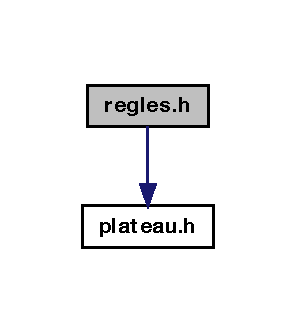
\includegraphics[width=142pt]{regles_8h__incl}
\end{center}
\end{figure}
Ce graphe montre quels fichiers incluent directement ou indirectement ce fichier :
\nopagebreak
\begin{figure}[H]
\begin{center}
\leavevmode
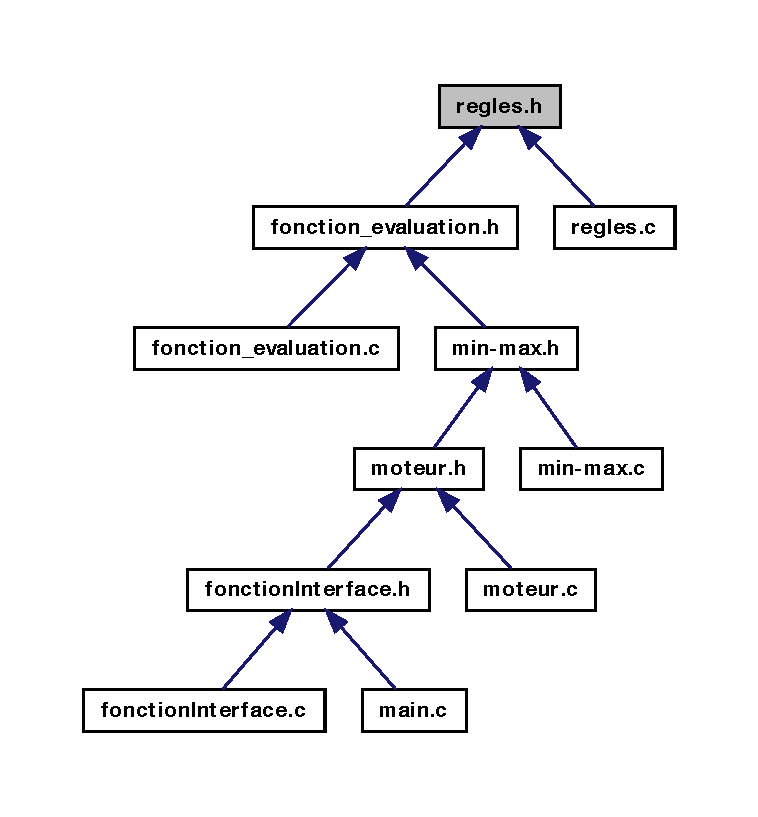
\includegraphics[width=364pt]{regles_8h__dep__incl}
\end{center}
\end{figure}
\subsection*{Fonctions}
\begin{DoxyCompactItemize}
\item 
\hyperlink{structcoup}{coup} $\ast$ \hyperlink{regles_8h_a96d861d76d7070b120ca385c13aad984}{coupsPossibles} (const \hyperlink{structcase__plateau}{case\_\-plateau} c, const \hyperlink{structplateau}{plateau} p)
\begin{DoxyCompactList}\small\item\em retourne le tableau des coups possible pour un coup donné. \item\end{DoxyCompactList}\item 
\hyperlink{structcoup}{coup} $\ast$ \hyperlink{regles_8h_a7c5456f7077282f58fc370d432ecdf73}{getCoups} (const \hyperlink{structjoueur}{joueur} j, const \hyperlink{structplateau}{plateau} p)
\begin{DoxyCompactList}\small\item\em retourne le tableau des coups possible pour le joueur donné. \item\end{DoxyCompactList}\item 
\hypertarget{regles_8h_a53ba636d2c102abd9c91db81bae620f4}{
\hyperlink{structcoup}{coup} $\ast$ {\bfseries getCoupsMax} (const \hyperlink{structcoup}{coup} $\ast$cp)}
\label{regles_8h_a53ba636d2c102abd9c91db81bae620f4}

\item 
\hyperlink{structcoup}{coup} $\ast$ \hyperlink{regles_8h_a8cad1d75ddb058fd96ae940dd593080e}{get\_\-deplacements} (const \hyperlink{structcase__plateau}{case\_\-plateau} c, const \hyperlink{structplateau}{plateau} p)
\begin{DoxyCompactList}\small\item\em retourne les deplacements possibles du pion de la case donné \item\end{DoxyCompactList}\item 
\hyperlink{structcoup}{coup} $\ast$ \hyperlink{regles_8h_a1bff1ac214ab2332d8b7e3a0b79f262c}{completer\_\-coup\_\-dame} (const \hyperlink{structcoup}{coup} c, int mvt, \hyperlink{structplateau}{plateau} p)
\item 
int \hyperlink{regles_8h_a69e7dc6de03ec30120b2a49ef6bb2f51}{get\_\-possible\_\-case\_\-pos} (int c, int diag, \hyperlink{structplateau}{plateau} p)
\item 
int \hyperlink{regles_8h_aec569c705e9ec403a06151aba2092c52}{compare\_\-coups} (\hyperlink{structcoup}{coup} $\ast$liste1, \hyperlink{structcoup}{coup} $\ast$liste2)
\item 
\hyperlink{structcase__plateau}{case\_\-plateau} \hyperlink{regles_8h_a60a8f706865d0ae9087f8d65d4667655}{get\_\-case\_\-plateau\_\-silent} (int x, int y, \hyperlink{structplateau}{plateau} p)
\begin{DoxyCompactList}\small\item\em retourne la case si elle existe, ou la case 0 sinon \item\end{DoxyCompactList}\end{DoxyCompactItemize}


\subsection{Description détaillée}
module des regles et d'enumeration des coups. \begin{DoxyAuthor}{Auteur}
Paraita Wohler 
\end{DoxyAuthor}


Définition dans le fichier \hyperlink{regles_8h_source}{regles.h}.



\subsection{Documentation des fonctions}
\hypertarget{regles_8h_aec569c705e9ec403a06151aba2092c52}{
\index{regles.h@{regles.h}!compare\_\-coups@{compare\_\-coups}}
\index{compare\_\-coups@{compare\_\-coups}!regles.h@{regles.h}}
\subsubsection[{compare\_\-coups}]{\setlength{\rightskip}{0pt plus 5cm}int compare\_\-coups (
\begin{DoxyParamCaption}
\item[{{\bf coup} $\ast$}]{liste1, }
\item[{{\bf coup} $\ast$}]{liste2}
\end{DoxyParamCaption}
)}}
\label{regles_8h_aec569c705e9ec403a06151aba2092c52}

\begin{DoxyParams}{Paramètres}
{\em liste1} & la premiere liste des coups \\
\hline
{\em liste2} & la seconde liste des coups \\
\hline
\end{DoxyParams}
\begin{DoxyReturn}{Renvoie}
0 si liste 1 == liste2, sinon 1 
\end{DoxyReturn}


Définition à la ligne \hyperlink{regles_8c_source_l00913}{913} du fichier \hyperlink{regles_8c_source}{regles.c}.

\hypertarget{regles_8h_a1bff1ac214ab2332d8b7e3a0b79f262c}{
\index{regles.h@{regles.h}!completer\_\-coup\_\-dame@{completer\_\-coup\_\-dame}}
\index{completer\_\-coup\_\-dame@{completer\_\-coup\_\-dame}!regles.h@{regles.h}}
\subsubsection[{completer\_\-coup\_\-dame}]{\setlength{\rightskip}{0pt plus 5cm}{\bf coup}$\ast$ completer\_\-coup\_\-dame (
\begin{DoxyParamCaption}
\item[{const {\bf coup}}]{c, }
\item[{int}]{mvt, }
\item[{{\bf plateau}}]{p}
\end{DoxyParamCaption}
)}}
\label{regles_8h_a1bff1ac214ab2332d8b7e3a0b79f262c}

\begin{DoxyParams}{Paramètres}
{\em mvt} & La diagonale du mouvement du coup précedent. \\
\hline
\end{DoxyParams}
\begin{DoxyReturn}{Renvoie}
La liste des coups possibles commençant par le coup c. 
\end{DoxyReturn}
\begin{DoxyAuthor}{Auteur}
Bastien Auda 
\end{DoxyAuthor}


Définition à la ligne \hyperlink{regles_8c_source_l00320}{320} du fichier \hyperlink{regles_8c_source}{regles.c}.

\hypertarget{regles_8h_a96d861d76d7070b120ca385c13aad984}{
\index{regles.h@{regles.h}!coupsPossibles@{coupsPossibles}}
\index{coupsPossibles@{coupsPossibles}!regles.h@{regles.h}}
\subsubsection[{coupsPossibles}]{\setlength{\rightskip}{0pt plus 5cm}{\bf coup}$\ast$ coupsPossibles (
\begin{DoxyParamCaption}
\item[{const {\bf case\_\-plateau}}]{c, }
\item[{const {\bf plateau}}]{p}
\end{DoxyParamCaption}
)}}
\label{regles_8h_a96d861d76d7070b120ca385c13aad984}


retourne le tableau des coups possible pour un coup donné. 


\begin{DoxyParams}{Paramètres}
{\em c} & La case qui contient le pion de la recherche. \\
\hline
{\em p} & la plateau courant. \\
\hline
\end{DoxyParams}


Définition à la ligne \hyperlink{regles_8c_source_l00024}{24} du fichier \hyperlink{regles_8c_source}{regles.c}.

\hypertarget{regles_8h_a60a8f706865d0ae9087f8d65d4667655}{
\index{regles.h@{regles.h}!get\_\-case\_\-plateau\_\-silent@{get\_\-case\_\-plateau\_\-silent}}
\index{get\_\-case\_\-plateau\_\-silent@{get\_\-case\_\-plateau\_\-silent}!regles.h@{regles.h}}
\subsubsection[{get\_\-case\_\-plateau\_\-silent}]{\setlength{\rightskip}{0pt plus 5cm}{\bf case\_\-plateau} get\_\-case\_\-plateau\_\-silent (
\begin{DoxyParamCaption}
\item[{int}]{x, }
\item[{int}]{y, }
\item[{{\bf plateau}}]{p}
\end{DoxyParamCaption}
)}}
\label{regles_8h_a60a8f706865d0ae9087f8d65d4667655}


retourne la case si elle existe, ou la case 0 sinon 


\begin{DoxyParams}{Paramètres}
{\em x} & la position horizontale sur le plateau \\
\hline
{\em y} & la position verticale sur le plateau \\
\hline
{\em p} & le plateau courant \\
\hline
\end{DoxyParams}
\begin{DoxyAuthor}{Auteur}
Paraita Wohler
\end{DoxyAuthor}

\begin{DoxyParams}{Paramètres}
{\em x} & la position en abscisse \\
\hline
{\em y} & la position en ordonnée \\
\hline
{\em p} & le plateau courant \\
\hline
\end{DoxyParams}
\begin{DoxyReturn}{Renvoie}
la case qui est en position x y dans p 
\end{DoxyReturn}


Définition à la ligne \hyperlink{regles_8c_source_l00929}{929} du fichier \hyperlink{regles_8c_source}{regles.c}.

\hypertarget{regles_8h_a8cad1d75ddb058fd96ae940dd593080e}{
\index{regles.h@{regles.h}!get\_\-deplacements@{get\_\-deplacements}}
\index{get\_\-deplacements@{get\_\-deplacements}!regles.h@{regles.h}}
\subsubsection[{get\_\-deplacements}]{\setlength{\rightskip}{0pt plus 5cm}{\bf coup}$\ast$ get\_\-deplacements (
\begin{DoxyParamCaption}
\item[{const {\bf case\_\-plateau}}]{c, }
\item[{const {\bf plateau}}]{p}
\end{DoxyParamCaption}
)}}
\label{regles_8h_a8cad1d75ddb058fd96ae940dd593080e}


retourne les deplacements possibles du pion de la case donné 


\begin{DoxyParams}{Paramètres}
{\em c} & la case ou est situé le pion dont on va chercher les déplacements possibles. \\
\hline
\end{DoxyParams}


Définition à la ligne \hyperlink{regles_8c_source_l00859}{859} du fichier \hyperlink{regles_8c_source}{regles.c}.

\hypertarget{regles_8h_a69e7dc6de03ec30120b2a49ef6bb2f51}{
\index{regles.h@{regles.h}!get\_\-possible\_\-case\_\-pos@{get\_\-possible\_\-case\_\-pos}}
\index{get\_\-possible\_\-case\_\-pos@{get\_\-possible\_\-case\_\-pos}!regles.h@{regles.h}}
\subsubsection[{get\_\-possible\_\-case\_\-pos}]{\setlength{\rightskip}{0pt plus 5cm}int get\_\-possible\_\-case\_\-pos (
\begin{DoxyParamCaption}
\item[{int}]{c, }
\item[{int}]{diag, }
\item[{{\bf plateau}}]{p}
\end{DoxyParamCaption}
)}}
\label{regles_8h_a69e7dc6de03ec30120b2a49ef6bb2f51}

\begin{DoxyParams}{Paramètres}
{\em c} & Notation officielle de la case de départ. \\
\hline
{\em diag} & Diagonale dans laquelle on recherche. \\
\hline
\end{DoxyParams}
\begin{DoxyReturn}{Renvoie}
0 si pas de cpions à prendre, la case sur laquelle se trouve le pion à prendre sinon. 
\end{DoxyReturn}


Définition à la ligne \hyperlink{regles_8c_source_l00249}{249} du fichier \hyperlink{regles_8c_source}{regles.c}.

\hypertarget{regles_8h_a7c5456f7077282f58fc370d432ecdf73}{
\index{regles.h@{regles.h}!getCoups@{getCoups}}
\index{getCoups@{getCoups}!regles.h@{regles.h}}
\subsubsection[{getCoups}]{\setlength{\rightskip}{0pt plus 5cm}{\bf coup}$\ast$ getCoups (
\begin{DoxyParamCaption}
\item[{const {\bf joueur}}]{j, }
\item[{const {\bf plateau}}]{p}
\end{DoxyParamCaption}
)}}
\label{regles_8h_a7c5456f7077282f58fc370d432ecdf73}


retourne le tableau des coups possible pour le joueur donné. 


\begin{DoxyParams}{Paramètres}
{\em j} & le joueur dont on chercher tout les coups \\
\hline
{\em p} & la plateau courant. \\
\hline
\end{DoxyParams}


Définition à la ligne \hyperlink{regles_8c_source_l00777}{777} du fichier \hyperlink{regles_8c_source}{regles.c}.


\hypertarget{regles_8h_source}{
\section{regles.h}
}

\begin{DoxyCode}
00001 
00006 \textcolor{comment}{/* ----------------------------------------------- */}
00007 
00008 \textcolor{preprocessor}{#include "\hyperlink{plateau_8h}{plateau.h}"}
00009 
00017 \hyperlink{structcoup}{coup}* coupsPossibles(\textcolor{keyword}{const} \hyperlink{structcase__plateau}{case_plateau} c, \textcolor{keyword}{const} \hyperlink{structplateau}{plateau} p);
00018 
00019 
00027 \hyperlink{structcoup}{coup}* getCoups(\textcolor{keyword}{const} \hyperlink{structjoueur}{joueur} j, \textcolor{keyword}{const} \hyperlink{structplateau}{plateau} p);
00028 
00029 
00036 \hyperlink{structcoup}{coup}* getCoupsMax(\textcolor{keyword}{const} \hyperlink{structcoup}{coup} *cp);
00037 
00038 
00045 \hyperlink{structcoup}{coup}* get\_deplacements(\textcolor{keyword}{const} \hyperlink{structcase__plateau}{case_plateau} c, \textcolor{keyword}{const} \hyperlink{structplateau}{plateau} p);
00046 
00047 
00054 \hyperlink{structcoup}{coup} * completer\_coup\_dame(\textcolor{keyword}{const} \hyperlink{structcoup}{coup} c, \textcolor{keywordtype}{int} mvt, \hyperlink{structplateau}{plateau} p);
00055 
00056 
00063 \textcolor{keywordtype}{int} get\_possible\_case\_pos(\textcolor{keywordtype}{int} c, \textcolor{keywordtype}{int} diag, \hyperlink{structplateau}{plateau} p) ;
00064 
00065 
00072 \textcolor{keywordtype}{int} compare\_coups(\hyperlink{structcoup}{coup} *liste1, \hyperlink{structcoup}{coup} *liste2);
00073 
00074 
00082 \hyperlink{structcase__plateau}{case_plateau} \hyperlink{plateau_8h_a60a8f706865d0ae9087f8d65d4667655}{get_case_plateau_silent}(\textcolor{keywordtype}{int} \hyperlink{plateau_8h_a9e00f85b4b6ec2d8bdfbe94ff40f0eeeacab1e15e82c5976bfb476ddfe145263c}{x}, \textcolor{keywordtype}{int} y, \hyperlink{structplateau}{plateau} p);
\end{DoxyCode}

\printindex
\end{document}
